\PassOptionsToPackage{unicode=true}{hyperref} % options for packages loaded elsewhere
\PassOptionsToPackage{hyphens}{url}
%
\documentclass[]{article}
\usepackage{lmodern}
\usepackage{amssymb,amsmath}
\usepackage{ifxetex,ifluatex}
\usepackage{fixltx2e} % provides \textsubscript
\ifnum 0\ifxetex 1\fi\ifluatex 1\fi=0 % if pdftex
  \usepackage[T1]{fontenc}
  \usepackage[utf8]{inputenc}
  \usepackage{textcomp} % provides euro and other symbols
\else % if luatex or xelatex
  \usepackage{unicode-math}
  \defaultfontfeatures{Ligatures=TeX,Scale=MatchLowercase}
\fi
% use upquote if available, for straight quotes in verbatim environments
\IfFileExists{upquote.sty}{\usepackage{upquote}}{}
% use microtype if available
\IfFileExists{microtype.sty}{%
\usepackage[]{microtype}
\UseMicrotypeSet[protrusion]{basicmath} % disable protrusion for tt fonts
}{}
\IfFileExists{parskip.sty}{%
\usepackage{parskip}
}{% else
\setlength{\parindent}{0pt}
\setlength{\parskip}{6pt plus 2pt minus 1pt}
}
\usepackage{hyperref}
\hypersetup{
            pdftitle={Simulating High-Dimensional Multivariate Data},
            pdfauthor={Alfred G. Schissler; Edward J. Bedrick; Alexander D. Knudson; Tomasz J. Kozubowski; Tin Nguyen; Anna K. Panorska; Juli Petereit; Walter W. Piegorsch; Duc Tran},
            pdfborder={0 0 0},
            breaklinks=true}
\urlstyle{same}  % don't use monospace font for urls
\usepackage[margin=1in]{geometry}
\usepackage{color}
\usepackage{fancyvrb}
\newcommand{\VerbBar}{|}
\newcommand{\VERB}{\Verb[commandchars=\\\{\}]}
\DefineVerbatimEnvironment{Highlighting}{Verbatim}{commandchars=\\\{\}}
% Add ',fontsize=\small' for more characters per line
\usepackage{framed}
\definecolor{shadecolor}{RGB}{248,248,248}
\newenvironment{Shaded}{\begin{snugshade}}{\end{snugshade}}
\newcommand{\AlertTok}[1]{\textcolor[rgb]{0.94,0.16,0.16}{#1}}
\newcommand{\AnnotationTok}[1]{\textcolor[rgb]{0.56,0.35,0.01}{\textbf{\textit{#1}}}}
\newcommand{\AttributeTok}[1]{\textcolor[rgb]{0.77,0.63,0.00}{#1}}
\newcommand{\BaseNTok}[1]{\textcolor[rgb]{0.00,0.00,0.81}{#1}}
\newcommand{\BuiltInTok}[1]{#1}
\newcommand{\CharTok}[1]{\textcolor[rgb]{0.31,0.60,0.02}{#1}}
\newcommand{\CommentTok}[1]{\textcolor[rgb]{0.56,0.35,0.01}{\textit{#1}}}
\newcommand{\CommentVarTok}[1]{\textcolor[rgb]{0.56,0.35,0.01}{\textbf{\textit{#1}}}}
\newcommand{\ConstantTok}[1]{\textcolor[rgb]{0.00,0.00,0.00}{#1}}
\newcommand{\ControlFlowTok}[1]{\textcolor[rgb]{0.13,0.29,0.53}{\textbf{#1}}}
\newcommand{\DataTypeTok}[1]{\textcolor[rgb]{0.13,0.29,0.53}{#1}}
\newcommand{\DecValTok}[1]{\textcolor[rgb]{0.00,0.00,0.81}{#1}}
\newcommand{\DocumentationTok}[1]{\textcolor[rgb]{0.56,0.35,0.01}{\textbf{\textit{#1}}}}
\newcommand{\ErrorTok}[1]{\textcolor[rgb]{0.64,0.00,0.00}{\textbf{#1}}}
\newcommand{\ExtensionTok}[1]{#1}
\newcommand{\FloatTok}[1]{\textcolor[rgb]{0.00,0.00,0.81}{#1}}
\newcommand{\FunctionTok}[1]{\textcolor[rgb]{0.00,0.00,0.00}{#1}}
\newcommand{\ImportTok}[1]{#1}
\newcommand{\InformationTok}[1]{\textcolor[rgb]{0.56,0.35,0.01}{\textbf{\textit{#1}}}}
\newcommand{\KeywordTok}[1]{\textcolor[rgb]{0.13,0.29,0.53}{\textbf{#1}}}
\newcommand{\NormalTok}[1]{#1}
\newcommand{\OperatorTok}[1]{\textcolor[rgb]{0.81,0.36,0.00}{\textbf{#1}}}
\newcommand{\OtherTok}[1]{\textcolor[rgb]{0.56,0.35,0.01}{#1}}
\newcommand{\PreprocessorTok}[1]{\textcolor[rgb]{0.56,0.35,0.01}{\textit{#1}}}
\newcommand{\RegionMarkerTok}[1]{#1}
\newcommand{\SpecialCharTok}[1]{\textcolor[rgb]{0.00,0.00,0.00}{#1}}
\newcommand{\SpecialStringTok}[1]{\textcolor[rgb]{0.31,0.60,0.02}{#1}}
\newcommand{\StringTok}[1]{\textcolor[rgb]{0.31,0.60,0.02}{#1}}
\newcommand{\VariableTok}[1]{\textcolor[rgb]{0.00,0.00,0.00}{#1}}
\newcommand{\VerbatimStringTok}[1]{\textcolor[rgb]{0.31,0.60,0.02}{#1}}
\newcommand{\WarningTok}[1]{\textcolor[rgb]{0.56,0.35,0.01}{\textbf{\textit{#1}}}}
\usepackage{longtable,booktabs}
% Fix footnotes in tables (requires footnote package)
\IfFileExists{footnote.sty}{\usepackage{footnote}\makesavenoteenv{longtable}}{}
\usepackage{graphicx,grffile}
\makeatletter
\def\maxwidth{\ifdim\Gin@nat@width>\linewidth\linewidth\else\Gin@nat@width\fi}
\def\maxheight{\ifdim\Gin@nat@height>\textheight\textheight\else\Gin@nat@height\fi}
\makeatother
% Scale images if necessary, so that they will not overflow the page
% margins by default, and it is still possible to overwrite the defaults
% using explicit options in \includegraphics[width, height, ...]{}
\setkeys{Gin}{width=\maxwidth,height=\maxheight,keepaspectratio}
\setlength{\emergencystretch}{3em}  % prevent overfull lines
\providecommand{\tightlist}{%
  \setlength{\itemsep}{0pt}\setlength{\parskip}{0pt}}
\setcounter{secnumdepth}{5}
% Redefines (sub)paragraphs to behave more like sections
\ifx\paragraph\undefined\else
\let\oldparagraph\paragraph
\renewcommand{\paragraph}[1]{\oldparagraph{#1}\mbox{}}
\fi
\ifx\subparagraph\undefined\else
\let\oldsubparagraph\subparagraph
\renewcommand{\subparagraph}[1]{\oldsubparagraph{#1}\mbox{}}
\fi

% set default figure placement to htbp
\makeatletter
\def\fps@figure{htbp}
\makeatother

% Place anything extra you'd like in the preamble
\usepackage{setspace}
\doublespacing
\usepackage{etoolbox}
\makeatletter
\providecommand{\subtitle}[1]{% add subtitle to \maketitle
  \apptocmd{\@title}{\par {\large #1 \par}}{}{}
}
\makeatother
\usepackage[]{natbib}
\bibliographystyle{plainnat}

\title{Simulating High-Dimensional Multivariate Data}
\providecommand{\subtitle}[1]{}
\subtitle{using the bigsimr R Package}
\author{Alfred G. Schissler \and Edward J. Bedrick \and Alexander D. Knudson \and Tomasz J. Kozubowski \and Tin Nguyen \and Anna K. Panorska \and Juli Petereit \and Walter W. Piegorsch \and Duc Tran}
\date{}

\begin{document}
\maketitle
\begin{abstract}
It is critical to realistically simulate data when conducting Monte Carlo studies and methods. But measurements are often correlated and high dimensional in this era of big data, such as data obtained through high-throughput biomedical experiments. Due to computational complexity and a lack of user-friendly software available to simulate these massive multivariate constructions, researchers may resort to simulation designs that posit independence or perform arbitrary data transformations. This greatly diminishes insights into the empirical operating characteristics of any proposed methodology, such as false positive rates, statistical power, interval coverage, and robustness. This article introduces the \texttt{bigsimr} R package that provides a flexible, scaleable procedure to simulate high-dimensional random vectors with given marginal characteristics and dependency measures. We'll describe the functions included in the package, including multi-core and graphical-processing-unit accelerated algorithms to simulate random vectors, estimate correlation, and find close positive semi-definite matrices. Finally, we demonstrate the power of \texttt{bigsimr} by applying these functions to our motivating dataset --- RNA-sequencing data obtained from breast cancer tumor samples with sample size \(n=1212\) patients and dimension \(d =1026\).
\end{abstract}

\hypertarget{introduction}{%
\section{Introduction}\label{introduction}}

Massive high-dimensional data sets are now commonplace in many areas of scientific inquiry.
As new methods are developed for these data, a fundamental challenge lies in designing and conducting simulation studies to assess the operating characteristics of proposed methodology, such as false positive rates, statistical power, interval coverage, and robustness --- often in comparison to existing methods.
Further, efficient simulation empowers statistical computing strategies, such as the parametric bootstrap \citep{Rizzo2007} to simulate from a hypothesized null model, providing inference in analytically challenging settings.
Such Monte Carlo (MC) techniques become difficult for high-dimensional data with the current existing algorithms and tools.
This is particularly true when simulating massive \emph{multivariate}, \emph{non-normal} distributions, arising naturally in many fields of study.

As others have noted, it can be vexing to simulate dependent, non-normal/discrete data --- even for low dimensional settings \citep{MB13, XZ19}.
For continuous non--normal multivariate data, the well-known NORmal To Anything (NORTA) algorithm \citep{Cario1997} and other copula \citep{Nelsen2007} approaches are well-studied with flexible, robust software available \citep{Yan2007, Chen2001}.
Yet these approaches do not scale in a timely fashion to high-dimensional problems \citep{Li2019gpu}.
For discrete data, early simulation strategies had major flaws --- such as failing to obtain the full range of possible dependencies (e.g., admitting only positive correlations \citet{Park1996}).
While more recent approaches \citep{MB13, Xia17, BF17} have largely remedied this issue for low-dimensional problems, the existing tools are not designed to scale to high dimensions.

Another central issue lies characterizing dependency between components in the high-dimensional random vector.
The choice of correlation in practice usually relates to the eventual analytic goal and distributional assumptions of the data (e.g.~non-normal, discrete, infinite support, etc).
For normal data, the Pearson product-moment correlation describes the dependency perfectly.
As we will see, however, simulating arbitrary random vectors that match a target Pearson correlation matrix exactly is computationally intense \citep{Chen2001, Xia17}.
On the other hand, an analyst may consider the use of nonparametric correlation measures to better characterize monotone, non-linear dependency, such as Spearman's \(\rho\) and Kendall's \(\tau\).
Throughout, we'll emphasize matching these nonparametric dependency measures as our aim lies in modeling non-normal data and these rank-based measures possess invariance properties favorable in our proposed methodology.

With all this mind, we present a scaleable, flexible multivariate simulation algorithm.
The crux of the method lies in the construction of a Gaussian copula, in the spirit of the NORTA procedure.
Further, we introduce the \texttt{bigsimr} R package that provides parallelized, high-performance software implemented our NORTA-inspired algorithm.
The algorithm design leverages useful properties of nonparametric correlation measures, namely invariance under monotone transformation and well-known closed form relationships between dependency measures for the multivariate normal (MVN) distribution.

The study proceeds by providing background information, including a description of our motivating example application --- RNA-sequencing (RNA-seq) breast cancer data.
Then we describe and justify our simulation methodology and related algorithms.
Next, we detail an illustrative low-dimensional example of basic and advanced use of the \texttt{bigsimr} R package.
Then we proceed with Monte Carlo studies under various distributional assumptions to assess accuracy and scaleable.
After the MC evaluations, we revisit our high-dimensional motivating example and employ our methods to commonplace statistical computing tasks.
Finally, we'll discuss the method's utility, limitations, and future directions.

\hypertarget{background}{%
\section{Background}\label{background}}

The \texttt{bigsimr} \texttt{R} package provides multiple algorithms to work with high-dimensional multivariate data, but all these algorithms were originally designed to support a single task:
to generate random vectors drawn from multivariate probability distribution with given marginal distributions and dependency metrics.
Specifically, our goal is to efficiently simulate a large number, \(B\), of random vectors \({\bf Y}=(Y_1, \ldots, Y_d)^\top\) with \textbf{correlated} components and heterogeneous marginal distributions, described via cumulative distribution functions (CDFs) \(F_i\), where \(d\) can be very large and still be computed in practically useful times.

When designing this methodology, we developed the following properties to guide our effort.
We divide the properties into two categories: (1) basic properties (BP) and ``scaleability'' properties (SP).
The BPs are adapted from an existing criteria due to \citet{Nik13a}.
Our simulation strategy should allow:

\begin{itemize}
\tightlist
\item
  BP1: A wide range of dependences, allowing both positive and negative values, and, ideally, admitting the full range of possible values.
\item
  BP2: Flexible dependence, meaning that the number of bivariate marginals can be equal to the number of dependence parameters.
\item
  BP3: Flexible marginal modeling, generating heterogeneous data --- possibly from differing probability families.
\end{itemize}

Moreover, the simulation method must \textbf{scale} to high dimensions:

\begin{itemize}
\tightlist
\item
  SP1: Procedure must scale to high dimensions, computable in a reasonable amount time.
\item
  SP2: Procedure must scale to high dimensions while maintaining accuracy.
\end{itemize}

To fix ideas and provide examples applications enabled via \texttt{bigsimr}, the next section describes a motivating data set that originally inspired the authors' interest in developing this methodology.

\hypertarget{motivating-example-rna-seq-data}{%
\subsection{Motivating example: RNA-seq data}\label{motivating-example-rna-seq-data}}

Simulating high-dimensional, non-normal, correlated data motivates this work --- in pursuit of modeling RNA-sequencing (RNA-seq) data \citep{Wang2009b, Conesa2016b} derived from breast cancer patients.
The RNA-seq data-generating process involves counting how often a particular messenger RNA (mRNA) is expressed in a biological sample.
RNA-seq platforms typically quantify the entire transcriptome in one experimental run, resulting in high-dimensional data.
For human derived samples, this results in count data corresponding to over 20,000 genes (protein-coding genomic regions) or even over 77,000 isoforms when alternatively-spliced mRNA are counted.
Importantly, due to inherent biological processes, gene expression data exhibits correlation --- co-expression --- across genes \citep{BE07, Schissler2018}.

We'll illustrate our methodology using the well-studied Breast Invasive Carcinoma (BRCA) data set housed in The Cancer Genome Atlas (TCGA; see Acknowledgments).
For simplicity, we only consider high expressing genes.
In turn, we begin by filtering to retain the top 5\% highest- expressing genes (in terms of median expression) of the 20,501 gene measurements from \(N=1212\) patients' tumor samples, resulting in \(d=1026\) genes.
This gives a massive number of pairwise dependencies among the marginals (specifically, \(\ensuremath{5.2582\times 10^{5}}\) correlation parameters).
We further process the data to illustrate our methodology's flexible and robust simulation scheme, while better aligning with the actual data-generating process, by rounding \citet{Li2011c} RNA-seq by Expectation Maximization (RSEM) values to counts.
Table \ref{tab:ch010-realDataTab} displays counts for three selected high-expressing genes for the first five patients' breast tumor samples.

\begin{table}

\caption{\label{tab:ch010-realDataTab}mRNA counts for three selected high-expressing genes from the first five observations of the BRCA data set.}
\centering
\begin{tabular}[t]{rrr}
\toprule
RPL5 & TXNIP & VIM\\
\midrule
20283 & 13401 & 26883\\
18614 & 11365 & 28806\\
31378 & 5365 & 22221\\
37861 & 5873 & 26871\\
17902 & 12564 & 15985\\
\bottomrule
\end{tabular}
\end{table}

To help visualize the bivariate relationships for these three selected genes across all patients, Figure \ref{fig:ch010-realDataFig} plots the marginal distributions and estimated Spearman's correlations (see Equation \eqref{eq:spearman} below).

\begin{figure}

{\centering 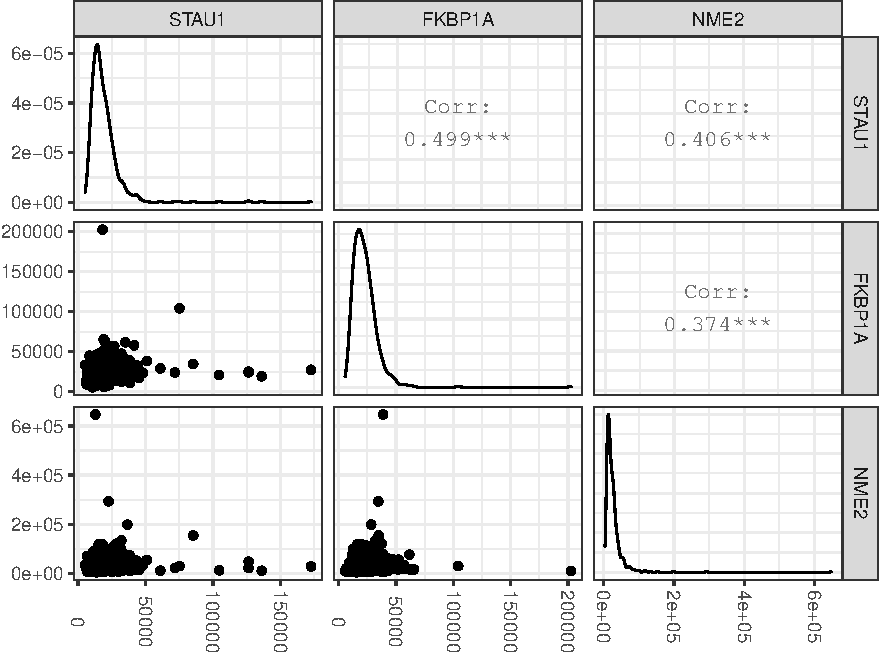
\includegraphics[width=0.85\linewidth]{article_bigsimr_files/figure-latex/ch010-realDataFig-1} 

}

\caption{Marginal scatterplots, densities, and estimated pairwise Spearman's correlations for three example genes. The data possess heavy-right tails, are discrete, and have non-trivial intergene correlations. Modeling these data motivate our simulation methodology.}\label{fig:ch010-realDataFig}
\end{figure}

\hypertarget{measures-of-dependency}{%
\subsection{Measures of dependency}\label{measures-of-dependency}}

In multivariate analysis, an analyst must select a metric to quantify dependency.
The most widely-known is the Pearson (product-moment) correlation coefficient that describes the linear association between two random variables \(X\) and \(Y\), and, it is given by

\begin{equation}
\label{eq:pearson}
\rho_P(X,Y) = \frac{E(XY) - E(X)E(Y)}{\left[ var(X)var(Y)\right]^{1/2}}.
\end{equation}

As \citet{MB13} and \citet{MK01} discuss, for a bivariate normal \((X,Y)\) random vector, the Pearson correlation completely describes the dependency between the components.
For non-normal marginals with monotone correlation patterns, \(\rho_P\) suffers some drawbacks and may mislead or fail to capture important relationships (\citet{MK01}).
Alternatively in these settings, analysts often prefer rank-based correlation measures to describe the degree of monotonic association.

Two nonparametric, rank-based measures common in practice are Spearman's correlation (denoted \(\rho_S\)) and Kendall's \(\tau\).
Define

\begin{equation}
\label{eq:spearman}
\rho_S(X,Y) = 3 \left[ P\left[ (X_1 - X_2)(Y_1-Y_3) > 0 \right] - P\left[ (X_1 - X_2)(Y_1-Y_3) < 0 \right] \right],
\end{equation}

\noindent where \((X_1, Y_1) \overset{d}{=} (X,Y), X_2 \overset{d}{=} X, Y_3 \overset{d}{=} Y\) with \(X_2\) and \(Y_3\) are independent of one other and of \((X_1, Y_1)\).
Spearman's \(\rho_S\) has an appealing correspondence as the Pearson's correlation coefficient on \emph{ranks} of the values, thereby captures nonlinear yet monotone relationships.

Kendall's \(\tau\), on the other hand, is the difference in probabilities of concordant and discordant pairs of observations \((X_i, Y_i)\) and \((X_j, Y_j)\).
By concordance we mean that orderings have the same direction (e.g., if \(X_i < X_j\), then \(Y_i < Y_j\)) and is determined by the ranks of the values, not the values themselves.

Both \(\tau\) and \(\rho_S\) are \textbf{invariant to under monotone transformations} of the underlying random variates.
As we will describe more fully in the \protect\hyperlink{algorithms}{Algorithms} section, this property is essential to scaleable match rank-based correlations with speed (SP1) and accuracy (SP2).

\emph{Correspondence among Pearson, Spearman, \(\tau\) correlations}.
This is no closed form, general correspondence among the rank-based measures and the Pearson correlation coefficient, as the marginal distributions \(F_i\) are intrinsic in their calculation.
But for \textbf{bivariate normal vectors}, however, the correspondence is well-known:

\begin{equation}
\label{eq:convertKendall}
\rho_{P} = sin \left( \tau \times \frac{\pi}{2} \right), 
\end{equation}

\noindent and similarly for Spearman's \(\rho\) \citep{K58},

\begin{equation}
\label{eq:convertSpearman}
\rho_P = 2 \times sin \left( \rho_S \times \frac{\pi}{6} \right).
\end{equation}

These facts are also critical in our simulation algorithm to broaden the dependency measures supported by \texttt{bigsimr}, in a computationally effective manner.

\emph{Discrete marginal considerations}.
Spearman's correlation for discrete marginal suffers some issues due to the nonzero probability of ties (for example, the Spearman's correlation of a discrete-valued random variable \(X\) with itself could be less than 1; \citet{MB13}).
One remedy for this issue is to rescale Equation \eqref{eq:spearman}.
For two random variables \(X,Y\) with probability mass functions (PMFs) or probability densities functions (PDFs) \(p(x)\) and \(q(y)\), respectively, define the rescaled Spearman's correlation as

\begin{equation}
\label{eq:spearmanRescaled}
\rho_{RS}(X,Y) = \frac{\rho_s(X,Y)}{ \left[ \left[ 1 - \sum_x p(x)^3 \right] \left[ 1 - \sum_y q(y)^3 \right] \right]^{1/2}}.
\end{equation}

Note that with continuous marginals the rescaling returns \(\rho_S\).
For discrete marginals with large or infinite support, computing the adjustment factors \(\sum_x p(x)^3\), \(\sum_y p(y)^3\) over all large number of pairs becomes expensive (often violating desired property SP1).
And further the infinite sums must be approximately for count-valued data and potentially violating desired property SP2.

Also, for a discrete random variable \(Y_i\), some care must be taken to define the quantile function \(F_{i}^{-1}\).
Let

\begin{equation}
F_{i}^{-1} = inf\{y:F_{i}(y) \geq u \}.
\label{eq:inverseCDF}
\end{equation}

\emph{Marginal-dependent bivariate correlation bounds}.
Given two marginal distributions, \(\rho_P\) is not free to vary the entire range of possible correlations \([-1,1]\).
The so-called \emph{Frechet-Hoeffding bounds} are well-studied (for example, see \citet{Nelsen2007} and \citet{BF17}).
This situation gives strict restraints on the possible correlations and cannot be overcome through algorithm design.
In general, the bounds are given by

\begin{equation}
\label{eq:frechet}
\rho_P^{max} = \rho_P \left( F^{-1}_1 (U), F^{-1}_2 (U) \right), \quad \rho_P^{min} = \rho_P \left( F^{-1}_1 (U), F^{-1}_2 (1 - U) \right)
\end{equation}

\noindent where \(U\) is a uniform random variable in \((0,1)\), and \(F^{-1}_1, F^{-1}_2\) are the inverse CDF of random variables \(X_1\) and \(X_2\), respectively.
For discrete random variables, define \(F^{-1}\) as in Equation \eqref{eq:inverseCDF}.

\hypertarget{gaussian-copulas}{%
\subsection{Gaussian copulas}\label{gaussian-copulas}}

There is a strong connection of our simulation strategy to Gaussian \textbf{copulas} (see \citet{Nelsen2007} for a technical introduction).
A copula is a distribution function on \([0,1]^d\) that describes a multivariate probability distribution with standard uniform marginals.
This definition provides a powerful, natural way characterize joint probability structure.
Consequently, the study of copulas is an important and active area of statistical theory and practice.

For any random vector \({\bf X}=(X_1, \ldots, X_d)\) with CDF \(F\) and marginal CDFs \(F_i\) there is a copula function
\(C(u_1, \ldots, u_d)\) so that

\[
F(x_1, \ldots,x_d) = \mathbb P(X_1\leq x_1, \ldots,X_d\leq x_d) = C(F_1(x_1), \ldots, F_d(x_d)), \,\,\, x_i\in \mathbb R, i=1,\ldots,d. 
\]

A Gaussian copula is the case where all marginal CDFs \(F_i\) are the standard normal CDF, \(\Phi\).
This representation corresponds to a multivariate normal distribution with standard normal marginal distributions and covariance matrix \({\bf R_P}\).
But since the marginals are standardized to have unit variance, this \({\bf R_P}\) is a Pearson correlation matrix.
If \(F_{{\bf R}}\) is the CDF of such a multivariate normal distribution, then the corresponding Gaussian copula \(C_{{\bf R}}\) is defined through

\begin{equation}
\label{eq:gauss}
F_{{\bf R}}(x_1, \ldots, x_d) = C_{{\bf R}}(\Phi(x_1), \ldots, \Phi(x_d)),
\end{equation}

where \(\Phi(\cdot)\) is the standard normal CDF.
Note that the copula \(C_{{\bf R}}\) is the familar multivariate normal CDF of the random vector \((\Phi(X_1), \ldots, \Phi(X_d))\), where \((X_1, \ldots, X_d) \sim N_d({\bf 0}, {\bf R_P})\).

Sklar's Theorem \citep{Sklar1959, Ubeda-Flores2017} guarantees that given inverse CDFs \(F_i^{-1}\)s and a valid correlation matrix (within the Frechet bounds) a random vector can be obtained via transformations involving copula functions.
For example, using Gaussian copulas, we can construct a random vector \({\bf Y} = (Y_1, \ldots, Y_d)\) with \(Y_i=F_i^{-1}(U_i)\), \(i=1, \ldots, d\), via \({\bf U} = (U_1, \ldots, U_d)\) viz \(U_i=\Phi(X_i)\), \(i=1, \ldots, d\) povides \(Y_i \sim F_i, \, \forall \, i\) .

\hypertarget{algorithms}{%
\section{Algorithms}\label{algorithms}}

This section describes our methods involved in simulating a random vector \(\bf Y\) with \(Y_i\) components for \(i=1,2,\ldots,d\).
Each \(Y_i\) has a specified marginal CDF \(F_i\) and its inverse \(F^{-1}_i\).
To characterize dependency, every pair \((Y_i, Y_j)\) has a given Pearson correlation \(\rho_P\), Spearman correlation \(\rho_S\), and/or Kendall's \(\tau\).
The method is best understand as a \textbf{high-performance Gaussian copula} (Equation \eqref{eq:gauss}) providing a high-dimensional NORTA-inspired algorithm.

\hypertarget{normal-to-anything-norta}{%
\subsection{NORmal To Anything (NORTA)}\label{normal-to-anything-norta}}

The well-known NORTA algorithm \citep{Cario1997} can be used simulate a random vector \(\bf Y\) with variance-covariance matrix \(\Sigma_{\bf Y}\).
Specifically, the NORTA algorithm follows like this:

\begin{enumerate}
\def\labelenumi{\arabic{enumi}.}
\tightlist
\item
  Simulate a random vector \(\bf Z\) with \(d\) \textbf{independent} and \textbf{identical} standard normal components.
\item
  Determine the input matrix \(\Sigma_{\bf Z}\) that corresponds with the specified output \(\Sigma_{\bf Y}\).
\item
  Produce a Cholesky factor \(M\) of \(\Sigma_{\bf Z}\) so that \(M M^{\prime}=\Sigma_{\bf Z}\).
\item
  Set \(X\) by \(X \gets MZ\).
\item
  \(\text{Return} \; Y \; \text{where} \; Y_i \gets F_{Y_i}^{-1}[\Phi(X_i)], \; i=1,2,...,d\).
\end{enumerate}

With modern parallelized computing, steps 1, 3, 4, 5 are readily implemented as high-performance, multi-core and/or graphical-processing-unit (GPU) accelerated, algorithms --- providing the fast scaleability using readily-available hardware.

Matching specified Pearson correlation coefficients exactly (step 2 above), however, is problematic.
In general, there is no closed form correspondence between the components of the input \(\Sigma_{\bf Z}\) and target \(\Sigma_{\bf Y}\).
Matching the correlations involves evaluating or approximating \(\binom{d}{2}\) integrals of the form \(EY_iY_j = \int \int y_i y_j f_{X}(F_i^{-1}(\Phi(z_i)), F_j^{-1}(\Phi(z_j))dy_idy_j\), for \(i,j=1,2,\ldots,d, \; i \neq j\).
For high-dimensional data, these evaluations are often too costly to enable feasible simulation studies.
For low-dimensional problems, methods and tools exist to match Pearson correlations precisely, see \citet{Chen2001}; \citet{Xia17}; \citet{MB13} and the publicly available \texttt{nortaRA} R package.

To maintain scaleability (SP1), our solution is to essentially avoid this complication in Pearson matching.
Since our goal is to simulate non-normal marginals, we greatly prefer the use of rank-based measures \(\rho_S\) and \(\tau\) from a modeling standpoint.
Further, \(\rho_S\) and \(\tau\)'s invariance under monotone transformation (see \protect\hyperlink{background}{Background}), preserves the correlation coefficients through steps 3, 4, and 5 in the NORTA algorithm above.
This eliminates the need for computing the \(\binom{d}{2}\) integrals to match exactly (nothing is for free, however, as discussed in below in Section \ref{rand-vec-gen}).

Despite all this, if one does desire to characterize dependency using Pearson correlations, simply using the target Pearson correlation matrix as the initial conditions to our proposed algorithm will lead to approximate matching in the resultant distribution \citep{Song00} in many practical applications.
The quality of this approximation depends on the setting, but in practice, for high-dimensional count data we find the accuracy to be adequate.
Later, we'll study the robustness of our method to this limitation in selected \href{\%7B\#simulations\%7D}{Monte Carlo evaluations}.

\hypertarget{rand-vec-gen}{%
\subsection{\texorpdfstring{Random vector generation via \texttt{bigsimr::rvec}}{Random vector generation via bigsimr::rvec}}\label{rand-vec-gen}}

Now we describe \texttt{bigsimr::rvec}, our algorithm to generate random vectors.
It mirrors the classical NORTA algorithm above with some modifications for rank-based dependency matching:

\begin{enumerate}
\def\labelenumi{\arabic{enumi}.}
\tightlist
\item
  Pre-processing for nonparametric dependency matching.

  \begin{enumerate}
  \def\labelenumii{(\roman{enumii})}
  \tightlist
  \item
    Convert from either \({\bf R_{Spearman}}\) or \({\bf R_{Kendall}}\) into the corresponding MVN input correlation \({\bf R_{Pearson}}\).
  \item
    Check that \({\bf R_{Pearson}}\) is semi-positive definite.\\
  \item
    If not compute a close semi-positive definite correlation matrix \({\bf \widetilde{R}_{Pearson}}\).\\
  \end{enumerate}
\item
  Gaussian copula construction.

  \begin{enumerate}
  \def\labelenumii{(\roman{enumii})}
  \tightlist
  \item
    Generate \({\bf X}=(X_1, \ldots, X_d) \sim N_d({\bf 0}, {\bf R_{Pearson}})\).\\
  \item
    Transform \({\bf X}\) to \({\bf U} = (U_1, \ldots, U_d)\) viz \(U_i=\Phi(X_i)\), \(i=1, \ldots, d\).\\
  \end{enumerate}
\item
  Quantile evaluations.

  \begin{enumerate}
  \def\labelenumii{(\roman{enumii})}
  \tightlist
  \item
    Return \({\bf Y} = (Y_1, \ldots, Y_d)\), where \(Y_i=F_i^{-1}(U_i)\), \(i=1, \ldots, d\);
  \end{enumerate}
\end{enumerate}

The pre-processing (Step 1) takes advantage of the closed-form relationships between \(\rho_S\) and \(\tau\) with \(\rho_P\) for bivariate normal random variables via Equations \eqref{eq:convertSpearman} or \eqref{eq:convertKendall}, respectively (implemented as \texttt{bigsimr::cor\_covert}).

A complication often arises at this stage: the resultant matrix may become indefinite, either through numerical error or naturally occurring in the correlation conversion.
Researchers working in multivariate computation frequently encounter such difficulties and need to find a close positive (semi-)definite matrix.
A widely-available routine for this task in \texttt{R} is called \texttt{matrix::nearPD}, though it is not suitable for high dimensions.
To overcome this issue, we've developed \texttt{bigsimr::nearPSD}, a quadractically-convergent Newton method for finding the nearest correlation matrix, developed by \citet{QS2006}.
We hope that this routine could be useful in many applications aside from our primary goal of random vector generation.

Once the target margins and algorithm inputs are determined, steps 2 and 3 are essentially a NORTA algorithm with modern high-performance computing implementations.
Specifically, step 2i uses either an efficient multi-core multivariate normal simulator (the \texttt{R} package \texttt{mvnfast}\citep{Fasiolo2016}) or a using Google's JAX python library NumPy for graphical-processing-unit (GPU) acceleration of the Cholesky factorization and matrix multiplication (steps 3, 4 in the NORTA algorithm in the preceding section).

\hypertarget{a-note-on-norta-in-higher-dimensions}{%
\subsection{A note on NORTA in higher dimensions}\label{a-note-on-norta-in-higher-dimensions}}

Sklar's theorem provides a useful characterization of multivariate distributions through copulas.
Yet the choice of copula-based simulation algorithm affects which joint distributions may be simulated.
Even in low-dimensional spaces (e.g., \(d=3\)), there exists valid multivariate distributions with \emph{feasible} Pearson correlation matrices that NORTA cannot match exactly \citep{LH75}.
This occurs when the bivariate transformations are applied to find the input correlation matrix yet when combined the resultant matrix is indefinite.
These situations do occur, even using exact analytic calculations. Such problematic target correlation matrices are termed \emph{NORTA defective}.

\citet{GH02} conducted a Monte Carlo study to estimate the probability of NORTA defective matrices while increasing the dimension \(d\).
They found at what is now considered low-to-moderate dimensions (\(d \approx 20\)) that almost \emph{all} feasible matrices are NORTA defective.
This stems from the concentration of measure near the boundary of the space of all possible correlation matrices as dimension increases. Unfortunately, it is precisely near this boundary that NORTA defective matrices reside.

There is hope, however, as \citet{GH02} also show that by augmenting the NORTA procedure by replacing the indefinite input correlation matrix with a close proxy will give approximate matching to the target --- with adequate performance for moderate \(d\).
This provides evidence that our nearest positive semi-definite (PSD) augmented approach will maintain reasonable accuracy if our input matching scheme returns an indefinite matrix, at least for the rank-based matching scheme described above.

\hypertarget{the-bigsimr-r-package}{%
\section{\texorpdfstring{The \texttt{bigsimr} R package}{The bigsimr R package}}\label{the-bigsimr-r-package}}

The \texttt{bigsimr} package is a high-performance implementation of the proposed random vector generation algorithm and associated functions (see Section \ref{algorithms} for details).
When designing \texttt{bigsimr}, we aimed to conveniently provide parallelized computation, through multi-core and GPU acceleration, while allowing advanced users to customize and automate workflows.

This subsections below describe the basic use of \texttt{bigsimr}, by stepping through a low-dimensional (2D) simulation workflow for the often-used example data set \texttt{airquality}.
This workflow proceeds from data, to estimation, simulation configuration, random vector generation, and result visualization.
For this low-dimensional setting, we compute using a single central processing unit (CPU) as the overhead in forking the tasks to multiple cores outweighs the computational gains.
Then we transition to advanced use where we briefly describe some of the high-performance features and syntax.
The section concludes with a short description of how to use \texttt{bigsimr} on a computer clusters through slurm scheduling via the \texttt{rslurm} package.

\hypertarget{basic-use-illustrated-through-a-minimal-example}{%
\subsection{Basic use illustrated through a minimal example}\label{basic-use-illustrated-through-a-minimal-example}}

We'll demonstrate the basic use and syntax of \texttt{bigsimr} through an example workflow applied to the New York air quality data set (\texttt{airquality}) included in the R \texttt{datasets} package.
First, we load the \texttt{bigsimr} library and a few other convenient data science packages, including the syntactically-elegant \texttt{tidyverse} suite of \texttt{R} packages.

\begin{Shaded}
\begin{Highlighting}[]
\KeywordTok{library}\NormalTok{(bigsimr)}
\KeywordTok{library}\NormalTok{(tidyverse)}
\KeywordTok{library}\NormalTok{(patchwork)}
\end{Highlighting}
\end{Shaded}

For simplicity and to provide a minimal working example, we'll consider bivariate simulation of temperature, in degrees Fahrenheit, and ozone level, in parts per billion.

\begin{Shaded}
\begin{Highlighting}[]
\NormalTok{df <-}\StringTok{ }\NormalTok{airquality }\OperatorTok
\StringTok{  }\KeywordTok{select}\NormalTok{(Temp, Ozone) }\OperatorTok
\StringTok{  }\KeywordTok{drop_na}\NormalTok{()}
\end{Highlighting}
\end{Shaded}

\begin{verbatim}
Rows: 116
Columns: 2
$ Temp  <int> 67, 72, 74, 62, 66, 65, 59, 61, 74, 69, 66, 68, 58, 64, 66, 5...
$ Ozone <int> 41, 36, 12, 18, 28, 23, 19, 8, 7, 16, 11, 14, 18, 14, 34, 6, ...
\end{verbatim}

Figure \ref{fig:ch030-aq-joint-dist} visualizes the bivariate relationship between Ozone and Temperature.
We aim to simulate random two-component vectors mimicking this structure.
The margins are not normally distributed, particularly the ozone level exhibits a strong positive skew.

\begin{figure}

{\centering 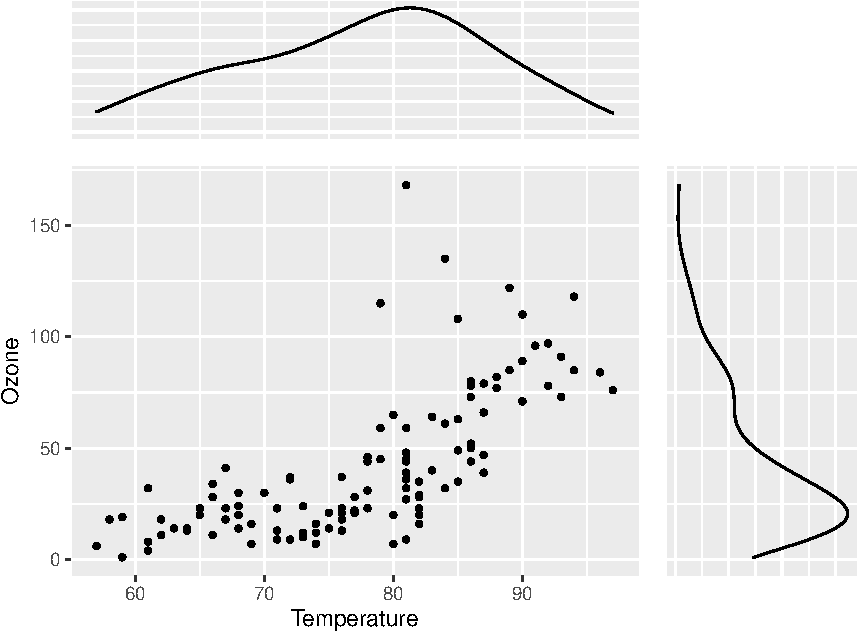
\includegraphics[width=0.85\linewidth]{article_bigsimr_files/figure-latex/ch030-aq-joint-dist-1} 

}

\caption{Bivariate scatterplot of Ozone vs. Temperature with estimated marginal densities. The data are left skewed tails and appear to be correlation.}\label{fig:ch030-aq-joint-dist}
\end{figure}

Next, we specify the marginal distributions and correlation coefficient (both its type and magnitude).
Here the analyst is free to be creative.
For this example, we will not take up goodness-of-fit considerations to determine the marginal distributions.
But it seems sensible without domain knowledge to estimate these quantities from the data and \texttt{bigsimr} contains fast functions designed for this task.

\emph{Specifying marginal distributions}.
Based on the estimated densities in Figure \ref{fig:ch030-aq-joint-dist}, we'll assume \texttt{Temp} is normally distributed and \texttt{Ozone} is log-normally distributed since its values are positive and skewed.
We'll use the well-known, unbiased estimators for the normal distribution's parameters and maximum likelihood estimators for the log-normal parameters:

\begin{Shaded}
\begin{Highlighting}[]
\NormalTok{df }\OperatorTok\StringTok{ }
\StringTok{  }\KeywordTok{select}\NormalTok{(Temp) }\OperatorTok\StringTok{ }
\StringTok{  }\KeywordTok{summarise_all}\NormalTok{(}\DataTypeTok{.funs =} \KeywordTok{c}\NormalTok{(}\DataTypeTok{mean =}\NormalTok{ mean, }\DataTypeTok{sd =}\NormalTok{ sd))}
\NormalTok{   mean    sd}
\DecValTok{1} \FloatTok{77.87} \FloatTok{9.485}
\end{Highlighting}
\end{Shaded}

\begin{Shaded}
\begin{Highlighting}[]
\NormalTok{mle_mean <-}\StringTok{ }\ControlFlowTok{function}\NormalTok{(x) }\KeywordTok{mean}\NormalTok{(}\KeywordTok{log}\NormalTok{(x))}
\NormalTok{mle_sd <-}\StringTok{ }\ControlFlowTok{function}\NormalTok{(x) }\KeywordTok{mean}\NormalTok{( }\KeywordTok{sqrt}\NormalTok{( (}\KeywordTok{log}\NormalTok{(x) }\OperatorTok{-}\StringTok{ }\KeywordTok{mean}\NormalTok{(}\KeywordTok{log}\NormalTok{(x)))}\OperatorTok{^}\DecValTok{2}\NormalTok{ ) )}

\NormalTok{df }\OperatorTok\StringTok{ }
\StringTok{  }\KeywordTok{select}\NormalTok{(Ozone) }\OperatorTok\StringTok{ }
\StringTok{  }\KeywordTok{summarise_all}\NormalTok{(}\DataTypeTok{.funs =} \KeywordTok{c}\NormalTok{(}\DataTypeTok{meanlog =}\NormalTok{ mle_mean, }\DataTypeTok{sdlog =}\NormalTok{ mle_sd))}
\NormalTok{  meanlog  sdlog}
\DecValTok{1}   \FloatTok{3.419} \FloatTok{0.6967}
\end{Highlighting}
\end{Shaded}

Next, we'll configure the input marginals for later input into \texttt{bigsimr::rvec}.
The marginal distributions are specifying using \texttt{R}'s special \texttt{alist} function.
This allows one to enter the distributions without evaluating anything (yet).

\begin{Shaded}
\begin{Highlighting}[]
\NormalTok{margins <-}\StringTok{ }\KeywordTok{alist}\NormalTok{(}
    \KeywordTok{qnorm}\NormalTok{(}\DataTypeTok{mean =} \FloatTok{77.871}\NormalTok{, }\DataTypeTok{sd =} \FloatTok{9.4855}\NormalTok{),}
    \KeywordTok{qlnorm}\NormalTok{(}\DataTypeTok{meanlog =} \FloatTok{3.419}\NormalTok{, }\DataTypeTok{sdlog =} \FloatTok{0.6967}\NormalTok{),}
\NormalTok{)}
\end{Highlighting}
\end{Shaded}

Notice that we use the \emph{quantile} function for the marginals, as that is how the marginal distributions \(F_i\) enter into the \texttt{bigsimr::rvec} algorithm.
This implementation strategy supports all \texttt{R} \texttt{base} probability distributions.
And allows flexible extensions using other \texttt{R} packages that adhere to conventions, such as \texttt{extraDistr}.
Further, by using \texttt{alist}, users can specify their own custom distributions (see below in \protect\hyperlink{custom-margins}{creating custom margins}).

It is a bit inconvenient to have to fill in the parameter values manually each time, so we provide a convenience function \texttt{mlist} which behaves similarly to \texttt{alist}, except that it will evaluate the right hand side of argument values within the list.
This is intended to help when scaling up your code to high dimensions when many marginals to specify.

\begin{Shaded}
\begin{Highlighting}[]
\NormalTok{margins <-}\StringTok{ }\KeywordTok{mlist}\NormalTok{(}
  \KeywordTok{qnorm}\NormalTok{(}\DataTypeTok{mean =} \KeywordTok{mean}\NormalTok{(df}\OperatorTok{$}\NormalTok{Temp), }\DataTypeTok{sd =} \KeywordTok{sd}\NormalTok{(df}\OperatorTok{$}\NormalTok{Temp)),}
  \KeywordTok{qlnorm}\NormalTok{(}\DataTypeTok{meanlog =} \KeywordTok{mle_mean}\NormalTok{(df}\OperatorTok{$}\NormalTok{Ozone), }\DataTypeTok{sdlog =} \KeywordTok{mle_sd}\NormalTok{(df}\OperatorTok{$}\NormalTok{Ozone))}
\NormalTok{)}
\NormalTok{margins}
\NormalTok{[[}\DecValTok{1}\NormalTok{]]}
\KeywordTok{qnorm}\NormalTok{(}\DataTypeTok{mean =} \FloatTok{77.8706896551724}\NormalTok{, }\DataTypeTok{sd =} \FloatTok{9.48548563759966}\NormalTok{)}

\NormalTok{[[}\DecValTok{2}\NormalTok{]]}
\KeywordTok{qlnorm}\NormalTok{(}\DataTypeTok{meanlog =} \FloatTok{3.41851510081201}\NormalTok{, }\DataTypeTok{sdlog =} \FloatTok{0.696668863646896}\NormalTok{)}
\end{Highlighting}
\end{Shaded}

\emph{Specifying correlation}.
As mentioned, the user must decide how to describe correlation, based on the particulars of the problem.
For non-normal data and for improved simulation accuracy in our scheme, we advocate the use of rank-based correlations Spearman's \(\rho_S\) and Kendall's \(\tau\).
But we also support approximate Pearson correlation coefficient matching, while cautioning the user to check the performance for their parametric multivariate model (see \protect\hyperlink{simulations}{Monte Carlo evaluations} for evaluation strategies and guidance).
To aid in correlation specification, and estimation in general, we provide a high-performance function \texttt{bigsimr::cor\_fast} which estimates Pearson, Spearman, or Kendall correlation using the fastest methods available.
(Anyone who has tried estimating Kendall's \(\tau\) using \texttt{stats::cor} can attest that the routine does not scale to even moderate dimensions).
Notably, these estimation methods are the standard approaches, not designed specifically designed for high-dimensional correlation estimation (see \href{\%7B\#discussion}{Conclusion and Discussion} for more on this).

\begin{Shaded}
\begin{Highlighting}[]
\NormalTok{type <-}\StringTok{ 'spearman'}
\NormalTok{(rho <-}\StringTok{ }\KeywordTok{cor_fast}\NormalTok{(df, }\DataTypeTok{method =} \StringTok{"spearman"}\NormalTok{))}
\NormalTok{       Temp Ozone}
\NormalTok{Temp  }\FloatTok{1.000} \FloatTok{0.774}
\NormalTok{Ozone }\FloatTok{0.774} \FloatTok{1.000}
\end{Highlighting}
\end{Shaded}

\emph{Checking the theoretical correlation bounds}
As discussed in Section \ref{background}, given a pair of marginal distributions the possible correlations are not free to vary between \([-1, 1]\).
To ensure that the simulation is not configured to impossible settings, we provide the \texttt{bigsimr::cor\_bounds} function provides MC estimated theoretical lower and upper bounds (using the Generate, Sort, and Correlate algorithm of \citet{DH2011}).

\begin{Shaded}
\begin{Highlighting}[]
\KeywordTok{cor_bounds}\NormalTok{(}\DataTypeTok{margins =}\NormalTok{ margins, }\DataTypeTok{type =}\NormalTok{ type)}
\OperatorTok{$}\NormalTok{lower}
\NormalTok{     [,}\DecValTok{1}\NormalTok{] [,}\DecValTok{2}\NormalTok{]}
\NormalTok{[}\DecValTok{1}\NormalTok{,]    }\DecValTok{1}   \DecValTok{-1}
\NormalTok{[}\DecValTok{2}\NormalTok{,]   }\DecValTok{-1}    \DecValTok{1}

\OperatorTok{$}\NormalTok{upper}
\NormalTok{     [,}\DecValTok{1}\NormalTok{] [,}\DecValTok{2}\NormalTok{]}
\NormalTok{[}\DecValTok{1}\NormalTok{,]    }\DecValTok{1}    \DecValTok{1}
\NormalTok{[}\DecValTok{2}\NormalTok{,]    }\DecValTok{1}    \DecValTok{1}
\end{Highlighting}
\end{Shaded}

Since our estimated Spearman correlation \(\hat{ \rho}_S\) is within the theoretical bounds, the correlation is valid as input to \texttt{bigsimr:rvec}.
On the other hand, the bounds on the Pearson correlation coefficient \(\rho_P\) between these margins is

\begin{Shaded}
\begin{Highlighting}[]
\KeywordTok{cor_bounds}\NormalTok{(}\DataTypeTok{margins =}\NormalTok{ margins, }\DataTypeTok{type =} \StringTok{'pearson'}\NormalTok{, }\DataTypeTok{reps=}\FloatTok{1e6}\NormalTok{)}
\OperatorTok{$}\NormalTok{lower}
\NormalTok{       [,}\DecValTok{1}\NormalTok{]   [,}\DecValTok{2}\NormalTok{]}
\NormalTok{[}\DecValTok{1}\NormalTok{,]  }\FloatTok{1.000} \FloatTok{-0.881}
\NormalTok{[}\DecValTok{2}\NormalTok{,] }\FloatTok{-0.881}  \FloatTok{1.000}

\OperatorTok{$}\NormalTok{upper}
\NormalTok{       [,}\DecValTok{1}\NormalTok{]   [,}\DecValTok{2}\NormalTok{]}
\NormalTok{[}\DecValTok{1}\NormalTok{,] }\FloatTok{1.0000} \FloatTok{0.8806}
\NormalTok{[}\DecValTok{2}\NormalTok{,] }\FloatTok{0.8806} \FloatTok{1.0000}
\end{Highlighting}
\end{Shaded}

\emph{Simulating random vectors}.
Finally, we arrive at the main function of \texttt{bigsimr}, \texttt{rvec}.
Let's now simulate \(B=10,000\) random vectors from the assumed joint distribution of Ozone levels and Temp.

\begin{Shaded}
\begin{Highlighting}[]
\NormalTok{x <-}\StringTok{ }\KeywordTok{rvec}\NormalTok{(}\DecValTok{10000}\NormalTok{, rho, margins, type)}
\NormalTok{df_sim <-}\StringTok{ }\KeywordTok{as.data.frame}\NormalTok{(x)}
\KeywordTok{colnames}\NormalTok{(df_sim) <-}\StringTok{ }\KeywordTok{colnames}\NormalTok{(df)}
\end{Highlighting}
\end{Shaded}

Figure \ref{fig:ch030-plot-sim} plots the 10,000 simulated points.

\begin{figure}

{\centering 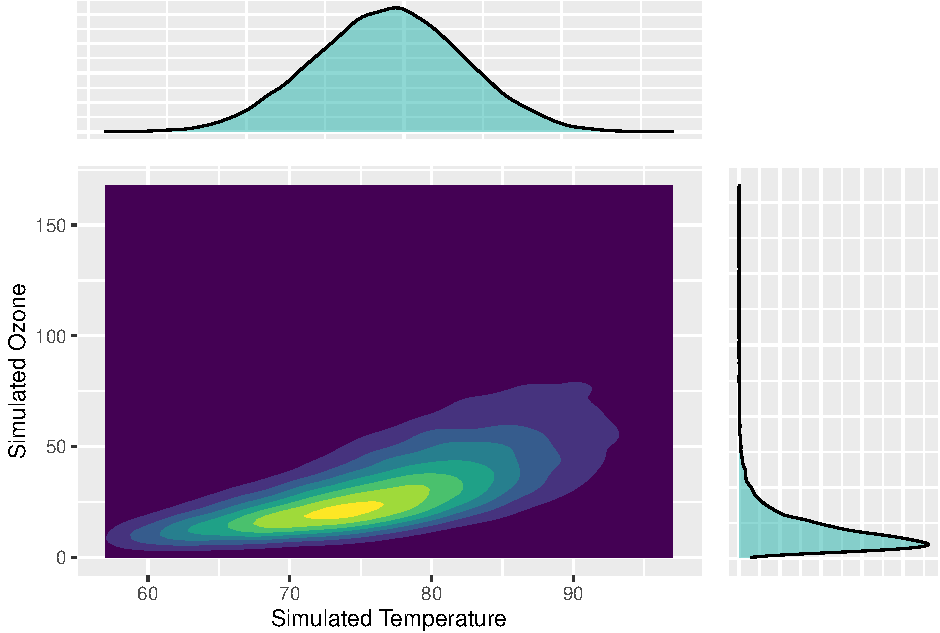
\includegraphics[width=0.85\linewidth]{article_bigsimr_files/figure-latex/ch030-plot-sim-1} 

}

\caption{Contour plot and marginal densities for the simulated bivariate distribution of Air Quality Temperatures and Ozone levels. The simulated points mimic the observed data with respect to both the marginal characteristics and bivariate association.}\label{fig:ch030-plot-sim}
\end{figure}

\hypertarget{advanced-use}{%
\subsection{Advanced use}\label{advanced-use}}

\emph{Creating a custom marginal distribution}.
Because \texttt{bigsimr} uses an \texttt{alist} to store the margins, any probability distribution with a well-defined inverse CDF can be used including custom marginal distributions not provided in base \texttt{R}.
Therefore, to specify a marginal distribution absent from an existing package, the user needs to provide a closed-form expression to form the corresponding quantile function.

It is important to follow \texttt{R}'s naming convention for probability distributions.
Users should prefix distributions with \texttt{r} and \texttt{q} for \emph{random} and \emph{quantile} respectively.
Only the quantile function is necessary to simulate random vectors, but to compute the theoretical correlation bounds, it is required to supply univariate random number generator as well.

For an example, let's provide a custom \emph{Pareto} distribution for use with \texttt{bigsimr}.
The Pareto CDF is

\[
F(x) = 1 - \left(\frac{x_m}{x}\right)^\alpha
\]

for scale \(x_m > 0\) and shape \(\alpha > 0\), with support \(x \in \left[x_m, \infty\right)\).
From the CDF, we compute the inverse CDF

\[
F^{-1}(p) = \frac{x_m}{\left(1 - p\right)^{1/\alpha}}
\]

Next we define the Pareto quantile function in R:

\begin{Shaded}
\begin{Highlighting}[]
\NormalTok{qpareto <-}\StringTok{ }\ControlFlowTok{function}\NormalTok{(p, scale, shape) \{}
\NormalTok{  scale }\OperatorTok{/}\StringTok{ }\NormalTok{(}\DecValTok{1} \OperatorTok{-}\StringTok{ }\NormalTok{p)}\OperatorTok{^}\NormalTok{(}\DecValTok{1}\OperatorTok{/}\NormalTok{shape)}
\NormalTok{\}}
\end{Highlighting}
\end{Shaded}

Writing random number generating function for our target marginal can be accomplished by calling the quantile function on a uniformly distributed random variable (the inverse transform method \citet{Rizzo2007}).

\begin{Shaded}
\begin{Highlighting}[]
\NormalTok{rpareto <-}\StringTok{ }\ControlFlowTok{function}\NormalTok{(n, scale, shape) \{}
  \KeywordTok{qpareto}\NormalTok{(}\KeywordTok{runif}\NormalTok{(n), scale, shape)}
\NormalTok{\}}
\end{Highlighting}
\end{Shaded}

Now with the \texttt{qpareto} and \texttt{rpareto} functions, we can use the distribution in \texttt{bigsimr} just like the other built-in distributions.

\begin{Shaded}
\begin{Highlighting}[]
\NormalTok{margins <-}\StringTok{ }\KeywordTok{alist}\NormalTok{(}
  \KeywordTok{qnorm}\NormalTok{(}\DataTypeTok{mean =} \FloatTok{3.14}\NormalTok{, }\DataTypeTok{sd =} \FloatTok{0.1}\NormalTok{),}
  \KeywordTok{qbeta}\NormalTok{(}\DataTypeTok{shape1 =} \DecValTok{1}\NormalTok{, }\DataTypeTok{shape2 =} \DecValTok{4}\NormalTok{),}
  \KeywordTok{qnbinom}\NormalTok{(}\DataTypeTok{size =} \DecValTok{10}\NormalTok{, }\DataTypeTok{prob =} \FloatTok{0.75}\NormalTok{),}
  \KeywordTok{qpareto}\NormalTok{(}\DataTypeTok{scale =} \FloatTok{1.11}\NormalTok{, }\DataTypeTok{shape =} \FloatTok{5.55}\NormalTok{)}
\NormalTok{)}
\KeywordTok{cor_bounds}\NormalTok{(margins, }\StringTok{"pearson"}\NormalTok{)}
\NormalTok{rho <-}\StringTok{ }\KeywordTok{cor_randPD}\NormalTok{(}\DecValTok{4}\NormalTok{)}
\NormalTok{x <-}\StringTok{ }\KeywordTok{rvec}\NormalTok{(}\DecValTok{10}\NormalTok{, rho, margins)}
\end{Highlighting}
\end{Shaded}

\emph{Using \texttt{bigsimr} on a computing cluster via \texttt{rslurm}}.
Though \texttt{bigsimr} runs quickly, at large \(d\) users may want to run jobs on a shared computing server.
The R package \texttt{rslurm} makes it easy to run embarrassingly large parallel \texttt{rvec} calls.
This example assumes that \texttt{bigsimr} is installed on a system with a slurm scheduler installed.
A single run of \texttt{bigsimr:rvec} using \texttt{rslurm} can be code as:

\begin{Shaded}
\begin{Highlighting}[]
\KeywordTok{library}\NormalTok{(rslurm)}
\NormalTok{sjob <-}\StringTok{ }\KeywordTok{slurm_call}\NormalTok{(rvec, }\DataTypeTok{jobname =} \StringTok{'rvec'}\NormalTok{,}
                   \KeywordTok{alist}\NormalTok{(}\DataTypeTok{n=}\FloatTok{1e6}\NormalTok{,}
                         \DataTypeTok{rho =}\NormalTok{ rho,}
                        \DataTypeTok{margins =}\NormalTok{ margins,}
                        \DataTypeTok{type =} \StringTok{"spearman"}\NormalTok{),}
                   \DataTypeTok{submit =} \OtherTok{TRUE}\NormalTok{)}
\end{Highlighting}
\end{Shaded}

Now, let's show off the real power of combining \texttt{bigsimr} and \texttt{rslurm} by simulating many correlation structures.
The \texttt{rslurm::slumr\_map} syntax mirrors the \texttt{base::lapply} and \texttt{purrr::map} functions.

\begin{Shaded}
\begin{Highlighting}[]
\KeywordTok{library}\NormalTok{(rslurm)}
\NormalTok{simReps <-}\StringTok{ }\DecValTok{100}
\NormalTok{rhoList <-}\StringTok{ }\KeywordTok{replicate}\NormalTok{( }\DataTypeTok{n =}\NormalTok{ simReps, bigsimr}\OperatorTok{::}\KeywordTok{cor_randPSD}\NormalTok{(}\DataTypeTok{d =} \KeywordTok{length}\NormalTok{(margins)),}
                     \DataTypeTok{simplify=}\OtherTok{FALSE}\NormalTok{ )}
\NormalTok{sjob <-}\StringTok{ }\KeywordTok{slurm_map}\NormalTok{(}\DataTypeTok{x =}\NormalTok{ rhoList,}
                  \DataTypeTok{f =}\NormalTok{ rvec,}
                  \DataTypeTok{jobname =} \StringTok{'rvecMap'}\NormalTok{,}
                  \DataTypeTok{n=}\FloatTok{1e6}\NormalTok{,}
                  \DataTypeTok{margins =}\NormalTok{ margins,}
                  \DataTypeTok{type =} \StringTok{"spearman"}\NormalTok{,}
                  \DataTypeTok{nodes =} \DecValTok{4}\NormalTok{,}
                  \DataTypeTok{cpus_per_node =} \DecValTok{4}\NormalTok{,}
                  \DataTypeTok{cores =} \DecValTok{4}\NormalTok{,}
                  \DataTypeTok{submit =} \OtherTok{TRUE}\NormalTok{)}
\end{Highlighting}
\end{Shaded}

On a cluster carrying 24 nodes with 48 threads, these 100 jobs completed in about a minute.

\hypertarget{simulations}{%
\section{Monte Carlo evaluations}\label{simulations}}

Before applying our methodology to real data simulation, we conduct several Monte Carlo studies to investigate method performance.
Since marginal parameter matching in our scheme is essentially a sequence of univariate inverse probability transforms, the challenging aspects are the accuracy of dependency matching and computational efficiency at high dimensions.
To evaluate our methods in those respects, we design the following numerical experiments to first assess accuracy in match dependency parameters in bivariate simulations and then time the procedure in increasingly large dimension \(d\).

\hypertarget{bivariate-experiments}{%
\subsection{Bivariate experiments}\label{bivariate-experiments}}

We select bivariate simulation configurations to ultimately simulate discrete-valued RNA-seq data and, so, proceed in increasing complexity, leading to the model in our motivating application in Section \ref{examples}.
We begin with empirically evaluating the dependency matching across all three supported correlations --- Pearson's, Spearman's, and Kendall's ---- in identical, bivariate marginal configurations.
For each pair of identical margins, we vary the correlations across the entire possible range of values to evaluate the simulation's ability to obtain the theoretic bounds.
The simulations progress from bivariate normal, to bivariate gamma (non-normal yet continuous), and bivariate negative binomial (mimicking RNA-seq counts).

Table \ref{tab:sims} lists our identical-marginal, bivariate simulation configurations.
We increase the simulate replicates \(B\) to check that our results converge to the target correlations and gauge statistical efficiency.
We select distributions beginning with a standard multivariate normal (MVN) as we expect the performance to be exact (up to MC error) for all correlation types.
Then, we select a non-symmetric continuous distribution: a standard (rate =1) two-component multivariate gamma (MVG).
Finally, we select distributions and marginal parameter values that are motivated by our RNA-seq data, namely values proximal to probabilities and sizes estimated from the data (see \href{examples}{Example applications for our motivating data} for estimation details).
Thus we arrive at a multivariate negative binomial (MVNB) \(p_1 = p_2 = \ensuremath{3\times 10^{-4}}, r_1 = r_2 = 4,\rho\) ).

\begin{longtable}[]{@{}lcr@{}}
\caption{\label{tab:sims} Identical margin, bivariate simulation configurations to evaluate correlation matching accuracy and efficiency.}\tabularnewline
\toprule
\begin{minipage}[b]{0.23\columnwidth}\raggedright
Simulation Reps (\(B\))\strut
\end{minipage} & \begin{minipage}[b]{0.28\columnwidth}\centering
Correlation Types\strut
\end{minipage} & \begin{minipage}[b]{0.40\columnwidth}\raggedleft
Identical-margin 2D distribution\strut
\end{minipage}\tabularnewline
\midrule
\endfirsthead
\toprule
\begin{minipage}[b]{0.23\columnwidth}\raggedright
Simulation Reps (\(B\))\strut
\end{minipage} & \begin{minipage}[b]{0.28\columnwidth}\centering
Correlation Types\strut
\end{minipage} & \begin{minipage}[b]{0.40\columnwidth}\raggedleft
Identical-margin 2D distribution\strut
\end{minipage}\tabularnewline
\midrule
\endhead
\begin{minipage}[t]{0.23\columnwidth}\raggedright
\(1000\)\strut
\end{minipage} & \begin{minipage}[t]{0.28\columnwidth}\centering
Pearson (\(\rho_P\))\strut
\end{minipage} & \begin{minipage}[t]{0.40\columnwidth}\raggedleft
\({ \bf Y} \sim MVN( \mu= 0 , \sigma = 1, \rho )\)\strut
\end{minipage}\tabularnewline
\begin{minipage}[t]{0.23\columnwidth}\raggedright
\(10,000\)\strut
\end{minipage} & \begin{minipage}[t]{0.28\columnwidth}\centering
Spearman (\(\rho_S\))\strut
\end{minipage} & \begin{minipage}[t]{0.40\columnwidth}\raggedleft
\({ \bf Y} \sim MVG( shape = 10, rate = 1, \rho )\)\strut
\end{minipage}\tabularnewline
\begin{minipage}[t]{0.23\columnwidth}\raggedright
\(100,000\)\strut
\end{minipage} & \begin{minipage}[t]{0.28\columnwidth}\centering
Kendall (\(\tau\))\strut
\end{minipage} & \begin{minipage}[t]{0.40\columnwidth}\raggedleft
\({ \bf Y} \sim MVNB(p = \ensuremath{3\times 10^{-4}}, r = 4,\rho)\)\strut
\end{minipage}\tabularnewline
\bottomrule
\end{longtable}

For each of the unique 9 simulation configurations above, we estimate the correlation bounds and vary \(\rho\) along a sequence of 100 points evenly placed within the bounds (minus an adjustment factor of \(\epsilon=0.01\) to handle numeric issues when the bound is specified exactly).

\begin{table}

\caption{\label{tab:ch040-biMAEtable}Average abolute error in matching the target dependency across the entire range of possible correlations for each bivariate marginal.}
\centering
\begin{tabular}[t]{lllr}
\toprule
No. of random vectors & Correlation type & Distribution & Mean abs. error\\
\midrule
1000 & Pearson & MVN & 0.0151\\
1000 & Pearson & MVG & 0.0217\\
1000 & Pearson & MVNB & 0.0326\\
\addlinespace
1000 & Spearman & MVN & 0.0182\\
1000 & Spearman & MVG & 0.0169\\
1000 & Spearman & MVNB & 0.0159\\
\addlinespace
1000 & Kendall & MVN & 0.0111\\
1000 & Kendall & MVG & 0.0122\\
1000 & Kendall & MVNB & 0.0114\\
\addlinespace
10000 & Pearson & MVN & 0.0055\\
10000 & Pearson & MVG & 0.0120\\
10000 & Pearson & MVNB & 0.0246\\
\addlinespace
10000 & Spearman & MVN & 0.0056\\
10000 & Spearman & MVG & 0.0056\\
10000 & Spearman & MVNB & 0.0050\\
\addlinespace
10000 & Kendall & MVN & 0.0040\\
10000 & Kendall & MVG & 0.0033\\
10000 & Kendall & MVNB & 0.0031\\
\addlinespace
1e+05 & Pearson & MVN & 0.0017\\
1e+05 & Pearson & MVG & 0.0102\\
1e+05 & Pearson & MVNB & 0.0227\\
\addlinespace
1e+05 & Spearman & MVN & 0.0017\\
1e+05 & Spearman & MVG & 0.0018\\
1e+05 & Spearman & MVNB & 0.0018\\
\addlinespace
1e+05 & Kendall & MVN & 0.0012\\
1e+05 & Kendall & MVG & 0.0011\\
1e+05 & Kendall & MVNB & 0.0010\\
\bottomrule
\end{tabular}
\end{table}

Figure \ref{fig:ch040-bPlot} displays the aggregated bivariate simulation results.
Table \ref{tab:ch040-biMAEtable} contains the mean absolute error (MAE) in reproducing the desired dependency measures for the three bivariate scenarios.
Taken together, the studies show our methodology is generally accuracy across the entire range of possible correlation values for the rank-based dependency measures, at least in these limited simulation settings for the rank-based correlations.
For the two non-normal bivariate marginals, the Pearson correlation matching is approximate.
For discrete margins, matching the dependency measures was somewhat less accurate, even for the rank-based metrics, and particularly inaccurate near the lower bound of Pearson correlations.

\begin{figure}

{\centering 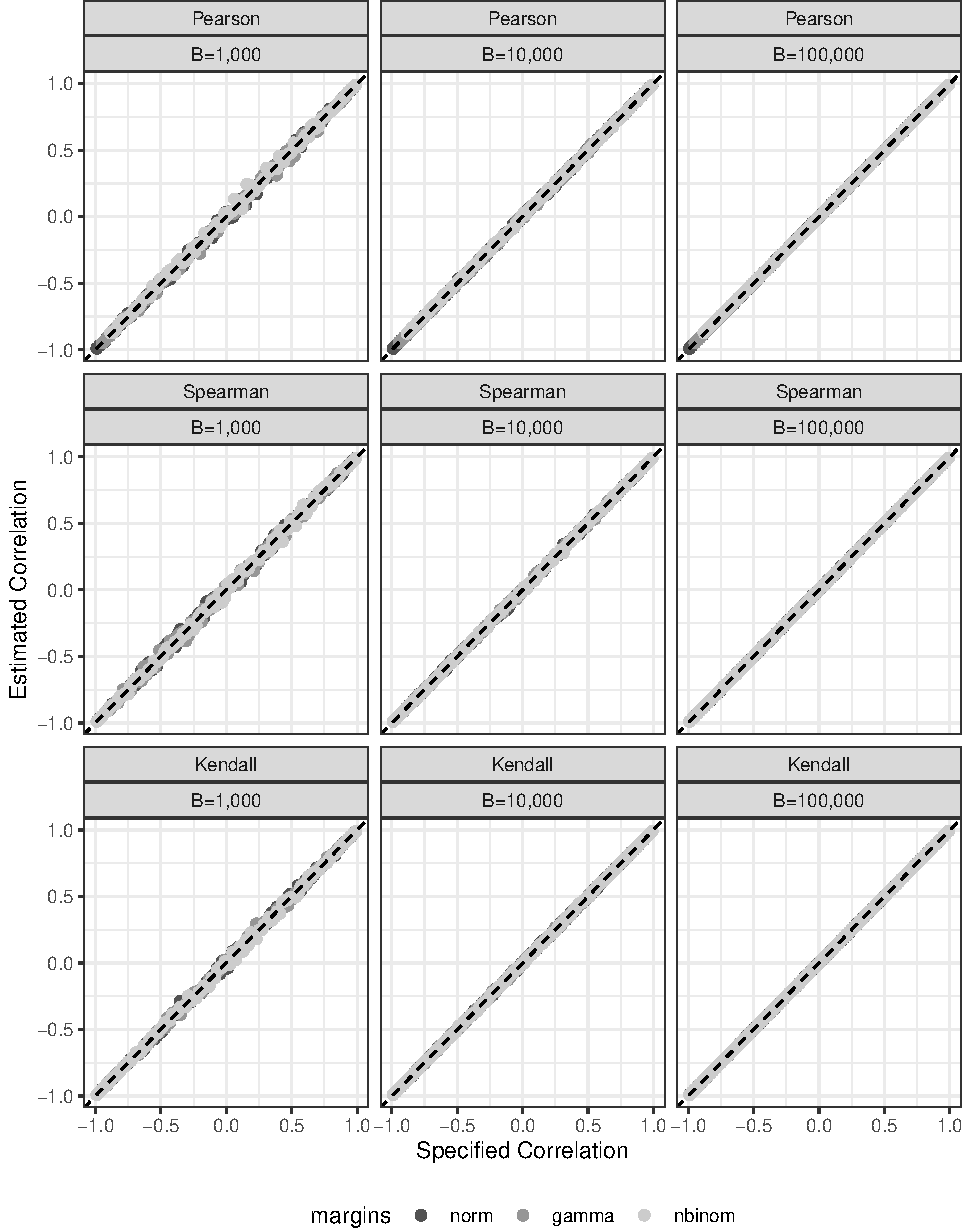
\includegraphics[width=0.85\linewidth]{article_bigsimr_files/figure-latex/ch040-bPlot-1} 

}

\caption{Bivariate simulations match specified correlations. The horizontal axis plots the specified target correlations across the entire range of possible correlations for each bivariate margin. Normal margins are plotted in dark blue, gamma in medium blue, and negative binomial in light blue. As the number of simulated vectors $B$ increases from left to right, the variation in estimated correlations (vertical axis) decreases. The dashed line indicates equality between the specified and estimated correlations. Only the normal margins match the Pearson correlations (top row) exactly across the entire range of correlations. The two non-normal bivariate random vectors experience attenuation (downward bias) for extreme Pearson correlations (due to limitations in our algorithm) and more restriction (due to the Frechet bounds). The rank-based correlations (bottom two rows) are matched exactly for all margins and obtain the full range of possible dependencies.}\label{fig:ch040-bPlot}
\end{figure}

The accuracy appears adequate for many applications.
In practice, we recommend users to always evaluate the accuracy for their application, using methods similar to those presented above.
See \href{discussion}{Discussion} for future directions for fast Pearson matching and discrete-specific modifications.

\hypertarget{scale-up-to-high-dimensions}{%
\subsection{Scale up to High Dimensions}\label{scale-up-to-high-dimensions}}

With information of our method's accuracy from a low-dimensional perspective, we now turn to assessing whether the \texttt{bigsimr} can scale to larger dimensional problems.
Specifically, we seek evidence to determine whether the method can scale to higher dimensions in a practical time.
Using our motivating RNA-seq data, described in \href{background}{Background}, we filtered the original 20,501 genes to the high-expressing genes at increasing percentiles, \(1, 5, 10, 15, 20, 25\%\), to obtain \(d=\{206, 1026, 2051, 3076, 4101, 5127\}\) marginals and \(\binom{d}{2}\) pairwise correlations at each setting.
For example, for \(d=5127\) there are \(13,140,501\) correlation coefficients.
We estimated the marginal negative binomial parameters and the correlation coefficients from the RNA-seq data to seed our simulations.
(See \href{examples}{Example applications for our motivating data} for a detailed description of estimation).

Figure \ref{fig:ch040-gpuVScpuFig} displays computation times using various high-performance settings (1 central processing unit, CPU-1, versus twenty CPUs, CPU-20; with and without GPU acceleration, GPU-1; GPU-20) to produce \(B=10,000\) random vectors.
The Pearson simulations are much faster since the correlation conversion steps are avoided (pre-processing step; see \href{algorithms}{Algorithms}), but as we know from above the accuracy will suffer slightly, especially near the negative boundary of the possible correlations.
Matching Spearman's correlation at larger \(d\) gets costly if one wants to produce \(B=10,000\) random vectors at many different simulation settings, but the conversion steps need only be computed once (see \href{MC-evaluation-of-correlation-estimation-efficiency}{MC evaluation of correlation estimation efficiency} for an example of this strategy).

\begin{figure}

{\centering 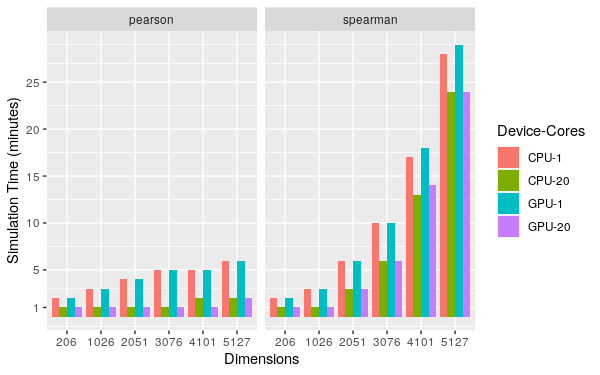
\includegraphics[width=0.8\linewidth]{fig/cpu-gpu-times} 

}

\caption{Computation times as d increases. We filter to the top 1, 5, 10, 15, 20, 25\% expressing genes (in terms of median expression.)}\label{fig:ch040-gpuVScpuFig}
\end{figure}

\hypertarget{examples}{%
\section{RNA-seq data example applications}\label{examples}}

This section demonstrates how to simulate multivariate data using \texttt{bigsimr}, aiming to replicate the structure of high-dimensional dependent count data.
In an illustration of our proposed methodology applied to real data, we seek to simulate RNA-sequencing data by producing simulated random vectors with assumed marginal distributions with estimated parameters that mimic the observed data and its generating process.
We seek scaleable realistic multivariate simulation to enable Monte Carlo (MC) methods for these data.
Modeling RNA-seq using multivariate probabilities distributions is natural as inter-gene correlation is an inherent part of biological processes.
Yet many models do not account for this, leading to major disruptions to the operating characteristics of statistical estimation, testing, and prediction.
See \citet{Efron2012} for a detailed discussion with related methods and see \citet{Wu2012b}, \citet{Schissler2018}, \citet{Schissler2019} for applied examples.
The following subsections apply \texttt{bigsimr}'s methods to real RNA-seq data, including replicated an estimated parametric structure, MC probability estimation, and MC evaluation of correlation estimation efficiency.

\hypertarget{simulating-high-dimensional-rna-seq-data}{%
\subsection{Simulating High-Dimensional RNA-seq data}\label{simulating-high-dimensional-rna-seq-data}}

Our first goal is to replicate the structure of the TCGA BRCA RNA-seq data set (see \href{background}{Background}).
Ultimately, we will simulate \(B=10,000\) random vectors \({\bf Y}=(Y_1, \ldots, Y_d)^\top\) with \(d=1026\).
Often researchers posit a negative binomial (NB) model as RNA-seq counts are often over-dispersed that a Poisson model would suggest.
All \(d\) selected genes exhibit over-dispersion (data not shown) and, so, we proceed to estimate the NB parameters \((r_i, p_i), i=1,\ldots,d\) to determine the target marginal PMFs \(f_i\) (via method of moments).
To complete specification of the simulation algorithm inputs, we'll estimate the Spearman correlation matrix \({ \bf R}_{Spearman}\) to characterize dependency.

With our goal in mind, we first estimate the desired correlation matrix using the fast implementation provided by \texttt{bigsimr}:

\begin{Shaded}
\begin{Highlighting}[]
\CommentTok{## Estimate Spearman's correlation on the count data}
\NormalTok{corType <-}\StringTok{ 'spearman'}
\KeywordTok{system.time}\NormalTok{( nb_Rho <-}\StringTok{ }\NormalTok{bigsimr}\OperatorTok{::}\KeywordTok{cor_fast}\NormalTok{( brca, }\DataTypeTok{method =}\NormalTok{ corType ) )}
\NormalTok{   user  system elapsed }
  \FloatTok{0.621}   \FloatTok{0.000}   \FloatTok{0.622} 
\end{Highlighting}
\end{Shaded}

Next, we estimate the marginal parameters.
We use method of moments (MoM) to estimate the marginal parameters for the multivariate negative binomial model.
The marginal distributions are from the same probability family (NB) yet are heterogeneous in terms of the parameters probability and size \((p_i, n_i)\) for \(i,\ldots,d\).
The functions below help achieve this estimation and specifying the inputs for use in \texttt{bigsimr::rvec}.

\begin{Shaded}
\begin{Highlighting}[]
\NormalTok{make_nbinom_alist <-}\StringTok{ }\ControlFlowTok{function}\NormalTok{(sizes, probs) \{}
  \KeywordTok{lapply}\NormalTok{(}\DecValTok{1}\OperatorTok{:}\KeywordTok{length}\NormalTok{(sizes), }\ControlFlowTok{function}\NormalTok{(i) \{}
    \KeywordTok{substitute}\NormalTok{(}\KeywordTok{qnbinom}\NormalTok{(}\DataTypeTok{size =}\NormalTok{ s, }\DataTypeTok{prob =}\NormalTok{ p), }
               \KeywordTok{list}\NormalTok{(}\DataTypeTok{s =}\NormalTok{ sizes[i], }\DataTypeTok{p =}\NormalTok{ probs[i]))}
\NormalTok{  \})}
\NormalTok{\}}
\CommentTok{## make_nbinom_alist(c(20, 21, 22), c(0.3, 0.4, 0.5))}
\NormalTok{nbinom_mom <-}\StringTok{ }\ControlFlowTok{function}\NormalTok{(x) \{}
\NormalTok{  m <-}\StringTok{ }\KeywordTok{mean}\NormalTok{(x)}
\NormalTok{  s <-}\StringTok{ }\KeywordTok{sd}\NormalTok{(x)}
\NormalTok{  s2 <-}\StringTok{ }\NormalTok{s}\OperatorTok{^}\DecValTok{2}
\NormalTok{  p <-}\StringTok{ }\NormalTok{m}\OperatorTok{/}\NormalTok{s2}
\NormalTok{  r <-}\StringTok{ }\NormalTok{m}\OperatorTok{^}\DecValTok{2} \OperatorTok{/}\StringTok{ }\NormalTok{(s2 }\OperatorTok{-}\StringTok{ }\NormalTok{m)}
  \KeywordTok{c}\NormalTok{(r, p)}
\NormalTok{\}}
\end{Highlighting}
\end{Shaded}

Now we estimate the marginal parameters using the built-in \texttt{apply}function:

\begin{Shaded}
\begin{Highlighting}[]
\NormalTok{sizes <-}\StringTok{ }\KeywordTok{apply}\NormalTok{( }\KeywordTok{unname}\NormalTok{(}\KeywordTok{as.matrix}\NormalTok{(brca)), }\DecValTok{2}\NormalTok{, nbinom_mom )[}\DecValTok{1}\NormalTok{, ]}
\NormalTok{probs <-}\StringTok{ }\KeywordTok{apply}\NormalTok{( }\KeywordTok{unname}\NormalTok{(}\KeywordTok{as.matrix}\NormalTok{(brca)), }\DecValTok{2}\NormalTok{, nbinom_mom )[}\DecValTok{2}\NormalTok{, ]}
\end{Highlighting}
\end{Shaded}

Notably, the marginal NB probabilities \(\hat{p}_i's\) are small --- ranging in \([\ensuremath{3.9342\times 10^{-6}} , 0.0122]\).
This gives rise to highly variable counts and, typically, less restriction on potential pairwise correlation pairs.
Once the functions are defined/executed to complete marginal estimation, we specify targets and generate the desired random vectors using \texttt{rvec}:

\begin{Shaded}
\begin{Highlighting}[]
\CommentTok{## Set the number of random vectors}
\NormalTok{n <-}\StringTok{ }\DecValTok{10000}
\CommentTok{## construct margins}
\NormalTok{nb_margins <-}\StringTok{ }\KeywordTok{make_nbinom_alist}\NormalTok{(sizes, probs)}
\CommentTok{## run sims}
\NormalTok{sim_nbinom <-}\StringTok{ }\KeywordTok{rvec}\NormalTok{(n, nb_Rho, nb_margins, }\DataTypeTok{type =}\NormalTok{ corType,}
                   \DataTypeTok{ensure_PSD =} \OtherTok{TRUE}\NormalTok{, }\DataTypeTok{cores =}\NormalTok{ cores) }
\KeywordTok{colnames}\NormalTok{(sim_nbinom) <-}\StringTok{ }\KeywordTok{names}\NormalTok{(brca)}
\end{Highlighting}
\end{Shaded}

Figure \ref{fig:ch050-simDataFig} displays the simulated counts and pairwise relationships for our example genes in Table \ref{tab:ch010-realDataTab}.
Simulated counts roughly mimic the observed data but with a smoother appearance due to the assumed parameter form and with less extreme points then the observed data (c.f. Figure \ref{fig:ch010-realDataFig}.)

\begin{figure}

{\centering 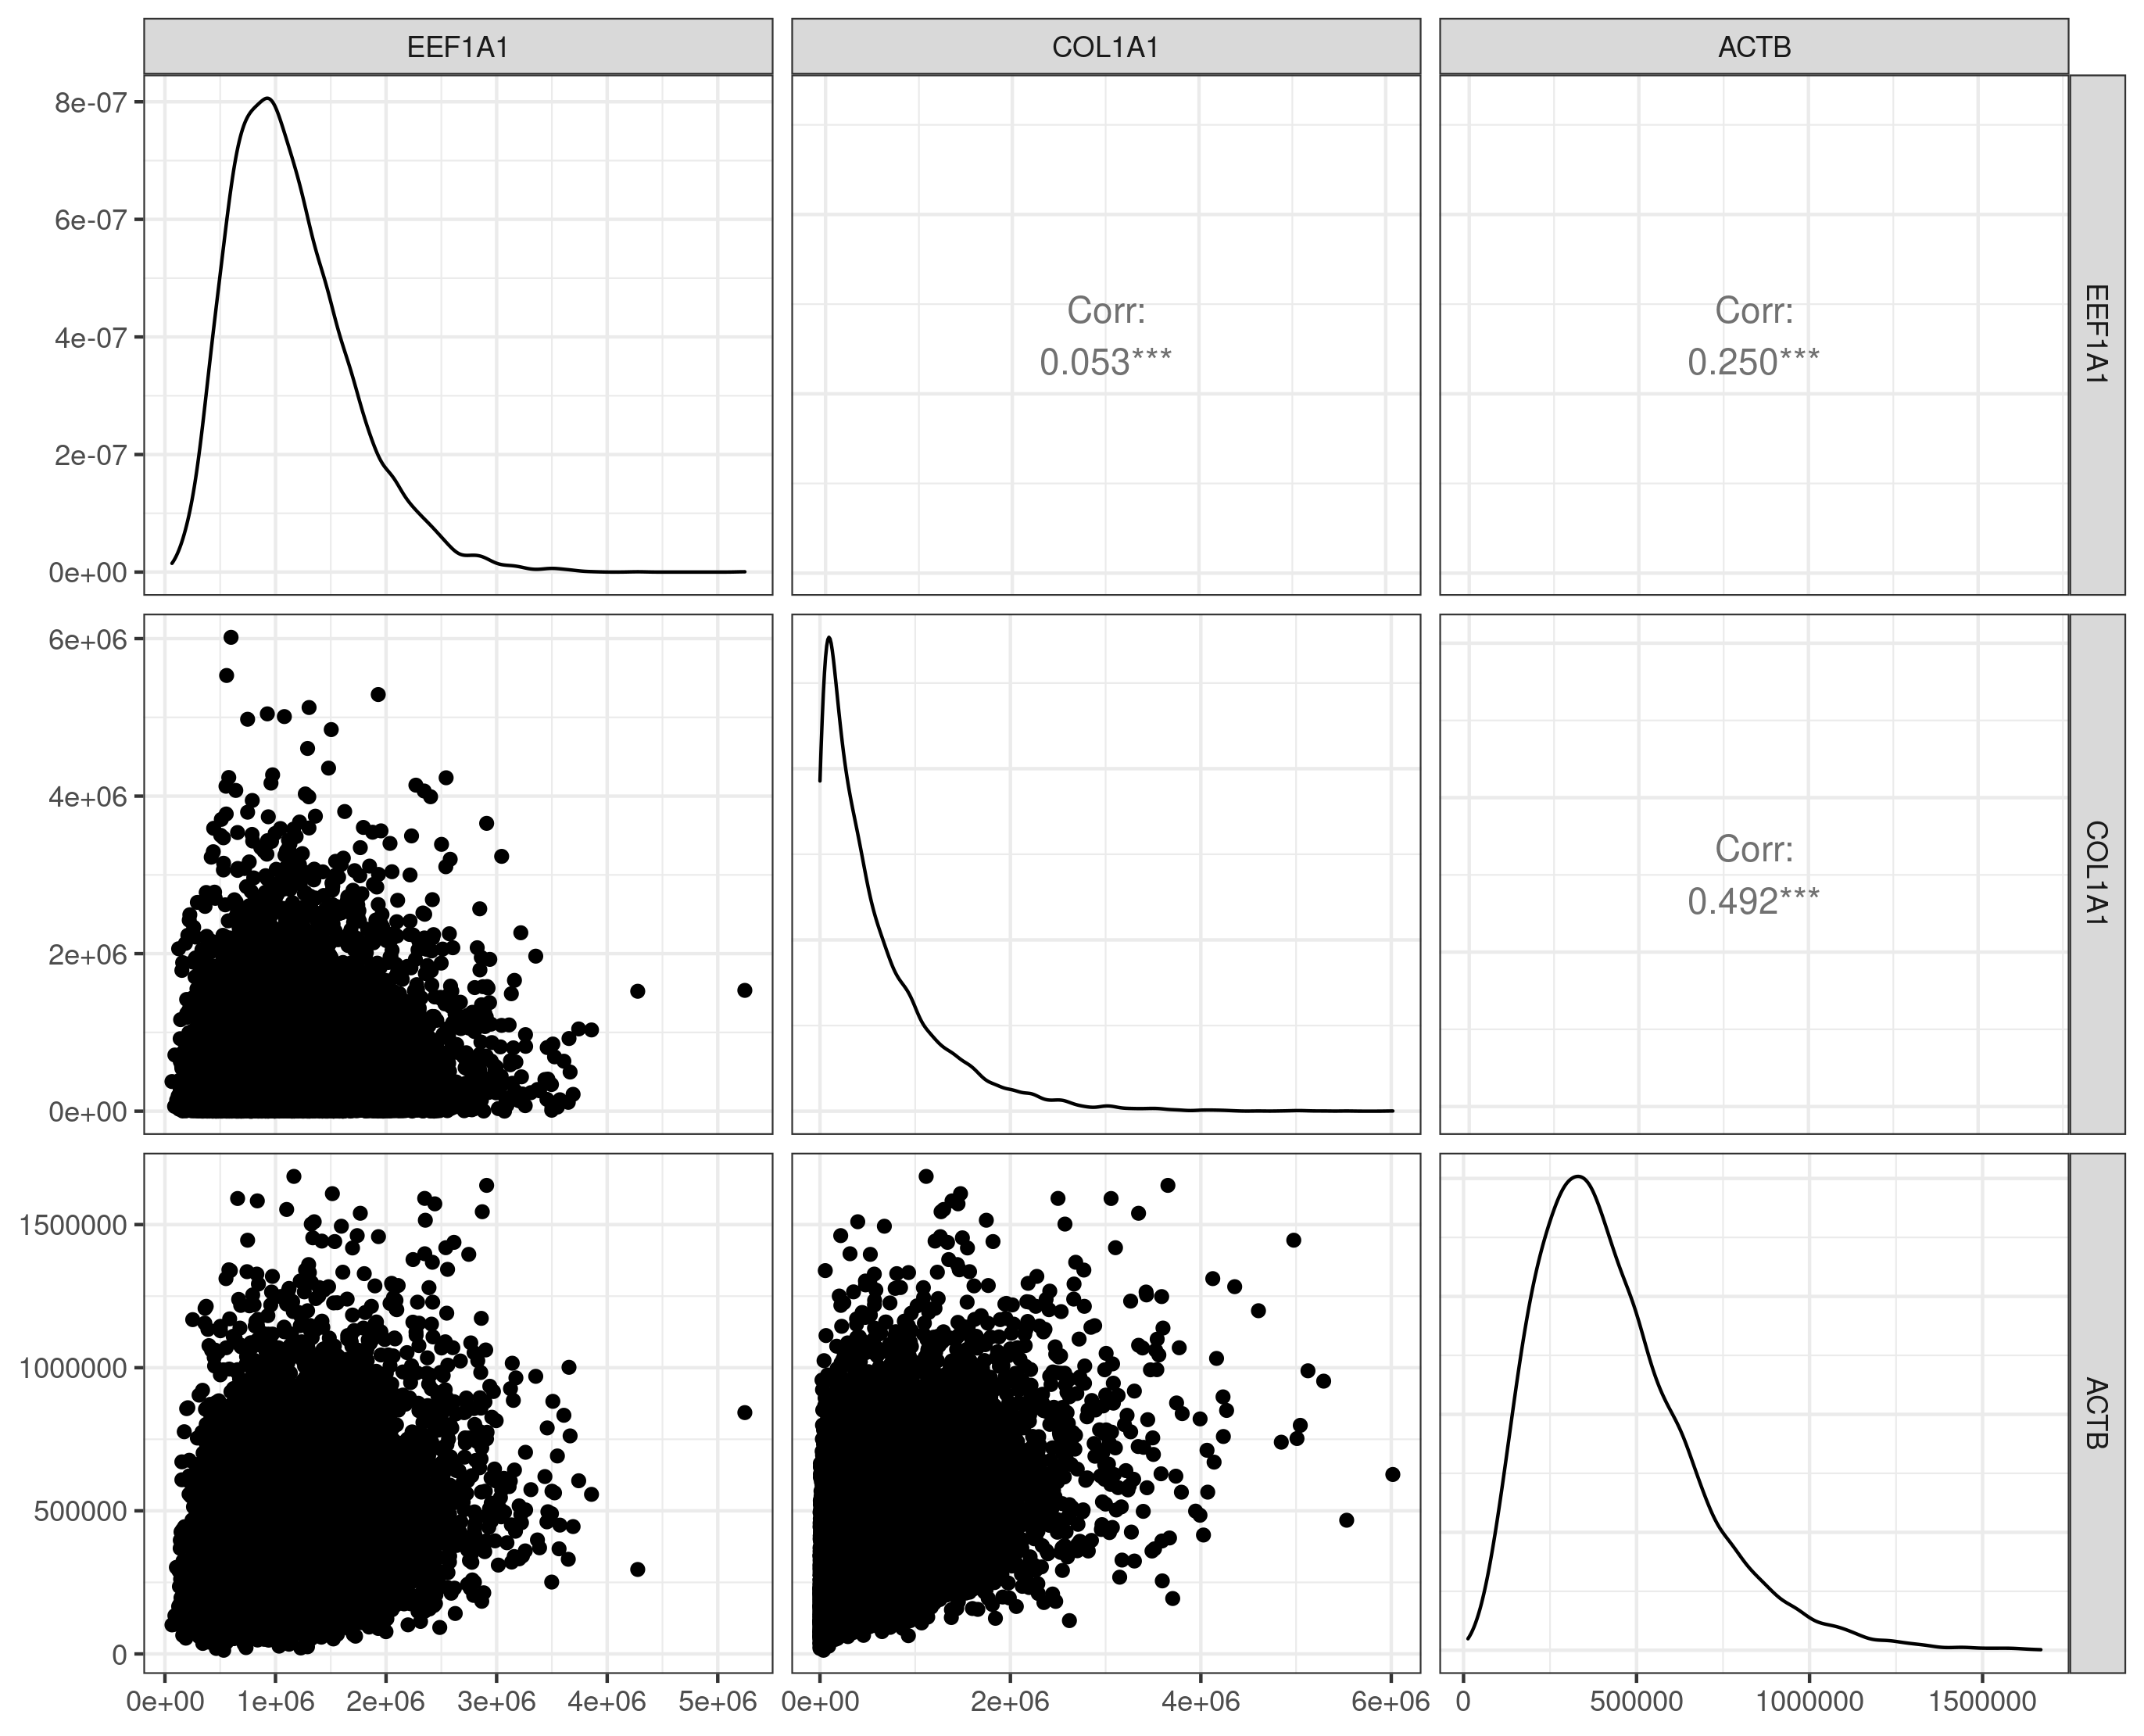
\includegraphics[width=0.85\linewidth]{fig/ch050-simDataFig} 

}

\caption{Simulated data for three selected high-expressing genes replicates the estimated data structure.}\label{fig:ch050-simDataFig}
\end{figure}

Figure \ref{fig:ch050-figBRCA} displays the aggregated results of our simulation by comparing the specified target parameter (horizontal axes) with the corresponding quantities estimated from the simulated data (vertical axes).
The evaluation shows that the simulated counts approximately match the target parameters and exhibit the full range of estimated correlation from the data.
Utilizing 15 CPU threads in a MacBook Pro carrying a 2.4 GHz 8-Core Intel Core i9 processor, the simulation completed just over of 2 minutes.

\begin{figure}

{\centering 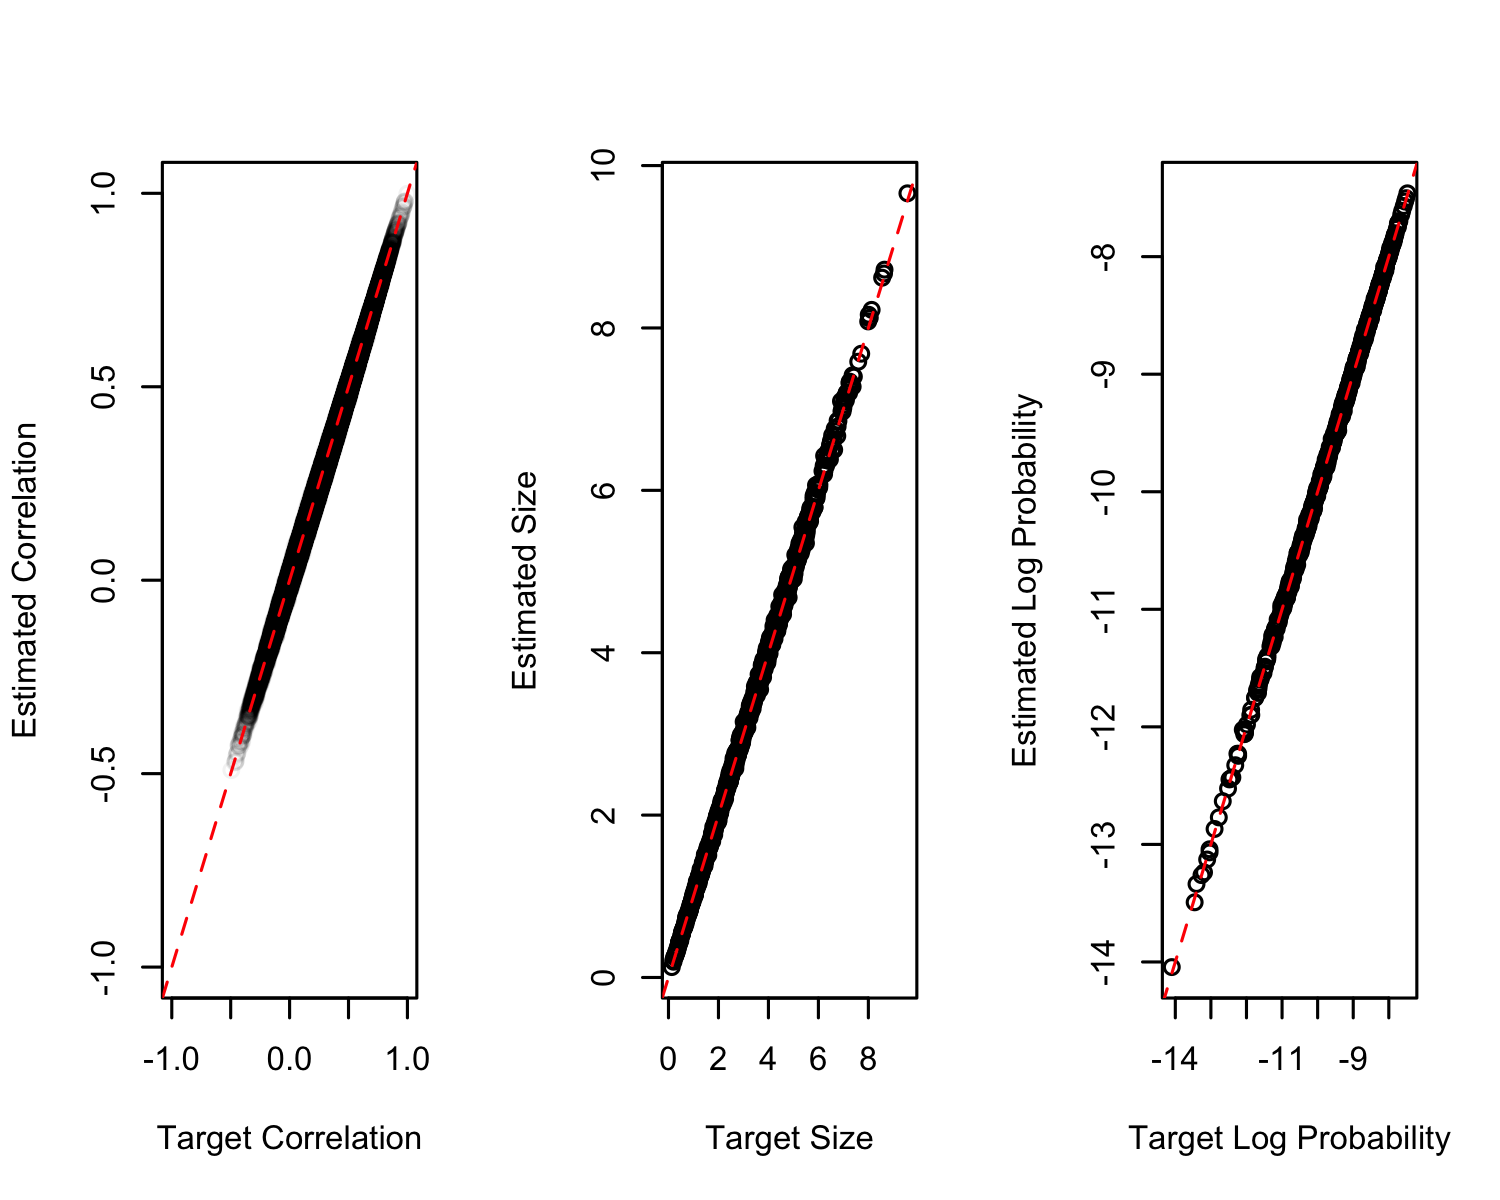
\includegraphics[width=0.8\linewidth]{fig/ch050-figBRCA} 

}

\caption{Simulated random vectors from a multivariate negative binomial replicate the estimated structure from an RNA-seq data set. The dashed red lines indicated equality between estimated parameters from simulated data (vertical axes) and the specified target parameters (horizontal axes).}\label{fig:ch050-figBRCA}
\end{figure}

\hypertarget{simulation-based-joint-probability-calculations}{%
\subsection{Simulation-based joint probability calculations}\label{simulation-based-joint-probability-calculations}}

To conduct statistical inference a critical task is to evaluate the joint probability mass (or density) function:

\[
P( {\bf Y} = {\bf y} ), y_i \in \chi_i.
\]

where \(\chi_i\) is the sample space for the \(i^{th}\) component of the random vector \(\bf{Y}\).
Compact representations with convenient computational forms are rare for high-dimensional constructions, especially with heterogeneous, correlated marginal distributions (or margins of mixed data types).
Given a large number simulated vectors as produced above, estimated probabilities are readily given by counting the proportion of simulated vectors meeting the desired condition.
In our motivating application, one may ask what is the probability that all genes expressed greater than a certain threshold value \({ \bf y}_0\).

Then we estimate

\[
\hat{P}( {\bf Y} >= {\bf y_0 } ) = \sum_{b=1}^B I( {\bf Y^{(b) }} > {\bf y_0 } ) / B
\]

where \({\bf Y^{(b)} }\) is the \(b^{th}\) simulated vector in a total of \(B\) simulation replicates and \(I ( )\) is the indicator function.
For example, we can estimate from our \(B=10,000\) simulated vectors the probability that all genes are expressed (i.e., \({\bf y}_i \geq 1, \forall \; i\)) is \(0.1708\).

\begin{Shaded}
\begin{Highlighting}[]
\NormalTok{d <-}\StringTok{ }\KeywordTok{ncol}\NormalTok{(sim_nbinom)}
\NormalTok{B <-}\StringTok{ }\KeywordTok{nrow}\NormalTok{(sim_nbinom)}
\NormalTok{threshold <-}\StringTok{ }\KeywordTok{rep}\NormalTok{( }\DecValTok{1}\NormalTok{, d)}
\KeywordTok{mean}\NormalTok{(}\KeywordTok{apply}\NormalTok{( sim_nbinom,  }\DecValTok{1}\NormalTok{,}
           \ControlFlowTok{function}\NormalTok{(X, }\DataTypeTok{y0=}\NormalTok{threshold) \{}
               \KeywordTok{all}\NormalTok{( X }\OperatorTok{>}\StringTok{ }\NormalTok{y0) \}}
\NormalTok{           ))}
\NormalTok{[}\DecValTok{1}\NormalTok{] }\FloatTok{0.1708}
\end{Highlighting}
\end{Shaded}

\hypertarget{evaluation-of-correlation-estimation-efficiency}{%
\subsection{Evaluation of correlation estimation efficiency}\label{evaluation-of-correlation-estimation-efficiency}}

MC methods are routinely used in many statistical inferential tasks including estimation, hypothesis testing, error rates, and empirical interval coverage rates.
For an concise introduction to these methods, see \citet{Rizzo2007}, Ch. 6.
To conclude the example applications, we demonstrate how \texttt{bigsimr} can be used evaluate estimation efficiency.
In particular, we'd like to assess the error in our correlation estimation above.
We used a conventional method, based on classical statistical theory.
Yet this method was not designed for high-dimensional data.
Indeed, high-dimensional covariance estimation (and precision matrices) is an active area of statistical science (see, for example, \citep{Won2013g, VanWieringen2016}.

In this small example, we simulate \(m=10\) data sets with the number of simulated vectors matching the number of patients in the BRCA data set, \(N=1212\).
Since our simulation is much faster for the Pearson correlation type (see Figure \ref{fig:ch040-gpuVScpuFig}), we only convert the Spearman correlation matrix once (and ensure its PSD).
At each iteration, we estimate the quadratic loss from the specified \({\bf R}_{Spearman}\), producing a distribution of loss values.

\begin{Shaded}
\begin{Highlighting}[]
\CommentTok{## Simulate random vectors equal to the sample size}
\NormalTok{n <-}\StringTok{ }\KeywordTok{nrow}\NormalTok{(brca)}
\CommentTok{## convert outside for faster simulation}
\NormalTok{nb_Rho_p <-}\StringTok{ }\NormalTok{bigsimr}\OperatorTok{::}\KeywordTok{cor_convert}\NormalTok{( }\DataTypeTok{rho =}\NormalTok{ nb_Rho,}
                                 \DataTypeTok{from =}\NormalTok{ corType, }\DataTypeTok{to =} \StringTok{"pearson"}\NormalTok{ )}
\CommentTok{## ensure PSD}
\NormalTok{nb_Rho_p <-}\StringTok{ }\NormalTok{bigsimr}\OperatorTok{::}\KeywordTok{cor_nearPSD}\NormalTok{( }\DataTypeTok{G =}\NormalTok{ nb_Rho_p )}
\CommentTok{## create m random vectors and estimate correlation}
\NormalTok{simRho <-}\StringTok{ }\KeywordTok{replicate}\NormalTok{(}\DataTypeTok{n =}\NormalTok{ m,}
  \DataTypeTok{expr =}\NormalTok{ \{ tmpSim <-}\StringTok{ }\KeywordTok{rvec}\NormalTok{(}\DataTypeTok{n =}\NormalTok{ n , nb_Rho_p, nb_margins,}
    \DataTypeTok{type =} \StringTok{'pearson'}\NormalTok{, }\DataTypeTok{ensure_PSD =} \OtherTok{FALSE}\NormalTok{, }\DataTypeTok{cores =}\NormalTok{ cores);}
\NormalTok{    bigsimr}\OperatorTok{::}\KeywordTok{cor_fast}\NormalTok{( }\DataTypeTok{x =}\NormalTok{ tmpSim, }\DataTypeTok{method =}\NormalTok{ corType )\} ,}
\DataTypeTok{simplify =} \OtherTok{FALSE}\NormalTok{)}
\CommentTok{## find quadratic loss at each rep}
\NormalTok{quadLoss <-}\StringTok{ }\KeywordTok{unlist}\NormalTok{( }\KeywordTok{lapply}\NormalTok{( simRho, rags2ridges}\OperatorTok{::}\NormalTok{loss,}
                           \DataTypeTok{T =}\NormalTok{ nb_Rho, }\DataTypeTok{type =} \StringTok{"quadratic"}\NormalTok{))}
\end{Highlighting}
\end{Shaded}

The \texttt{R} summary function supplies the mean-augmented five-number summary of the quadratic loss distribution computed above.

\begin{Shaded}
\begin{Highlighting}[]
\KeywordTok{summary}\NormalTok{(quadLoss)}
\NormalTok{   Min. 1st Qu.  Median    Mean 3rd Qu.    Max. }
\DecValTok{1225076} \DecValTok{1251629} \DecValTok{1277417} \DecValTok{1321153} \DecValTok{1390574} \DecValTok{1461040} 
\end{Highlighting}
\end{Shaded}

This distribution could be compared to high-dimensional designed covariance estimators to guide to help decide whether the additional complexity and computation time are warranted.

\hypertarget{discussion}{%
\section{Conclusion and discussion}\label{discussion}}

We've introduced a general-purpose high-dimensional multivariate simulation algorithm and provide a high-performance \texttt{R} package called \href{https://schisslergroup.github.io/bigsimr/}{\texttt{bigsimr}}.
The random vector generation method is largely inspired by NORTA (\citet{Cario1997}) and Gaussian copula-based approaches (\citet{MB13}, \citet{BF17}, \citet{Xia17}).
The major contributions of this work are high-dimensional scaleability, flexible modeling of dependency, and an high-performance implementation with broad potential data analytic applications for modern, big-data statistical computing.

It is customary to compare new tools and algorithms directly to existing competing methods and software.
In this study, however, we only employ our proposed methodology, since our previous work has show that existing tools are simply not designed or feasible to meet our high-dimensional goal (see \citet{Li2019gpu} for evaluations of the \texttt{R} \texttt{copula}package and others).
For the bivariate simulations, existing packages such as \href{https://github.com/cran/NORTARA/blob/master/inst/doc/NORTARA.R}{\texttt{nortaRA}} work well to match Pearson correlations exactly.

There are limitations to the methodology and implementation.
The most obvious missing feature of the proposed methodology is the inability to match a Pearson correlation matrix exactly.
As discussed in \href{algorithms}{Algorithms} and extensively by \citet{XZ19}, this is a computationally intense procedure and Pearson's correlation is not a natural choice to describe dependency for non-normal marginals.
While we do not provide an implementation directly supporting Pearson matching, users may supply their own input Pearson correlation after using a supplementary matching scheme \citep{Cario1997, XZ19}.

Future work includes developing scaleable algorithms to match the Pearson correlation matrix more precisely, discrete-margin specific modifications including fast Spearman's correlation rescaling (see Equation \eqref{eq:spearmanRescaled}), and high-dimensional covariance estimation.
From an implementation standpoint, \texttt{bigsimr} only supports Nvidia GPUs and redesigning the code using OpenCL would broaden the users who would benefit.
As data-analytic problems grow to even larger dimension, multi-GPU support is a promising hardware-based future direction.

\hypertarget{misc}{%
\section*{Supplementary Materials}\label{misc}}
\addcontentsline{toc}{section}{Supplementary Materials}

We provide an open-source implementation of our methodology as the \texttt{bigsimr} R package, hosted on github, \url{https://schisslergroup.github.io/bigsimr/}.

\begin{center}
\includegraphics[width=0.05\linewidth]{images/hex-bigsimr} \end{center}

\hypertarget{acknowledgments}{%
\section*{Acknowledgment(s)}\label{acknowledgments}}
\addcontentsline{toc}{section}{Acknowledgment(s)}

The authors gratefully acknowledge the helpful discussions with University of Arizona's Professor Walter W. Piegorsch and Professor Edward J. Bedrick during this project's conception.
We also gratefully acknowledge Heather Knudson's graphic design for the \texttt{bigsimr} R Package.
The results published here are in whole or part based upon data generated by the TCGA Research Network: \url{https://www.cancer.gov/tcga}.

\hypertarget{coi}{%
\section*{Disclosure statement}\label{coi}}
\addcontentsline{toc}{section}{Disclosure statement}

The authors report no conflict of interest.

\hypertarget{funding}{%
\section*{Funding}\label{funding}}
\addcontentsline{toc}{section}{Funding}

Research reported in this publication was supported by MW-CTR-IN of the National Institutes of Health under award number NIH 1U54GM104944.

\bibliography{bigsimr.bib,packages.bib}

\end{document}
